\documentclass{beamer}

%For final version: remove the [draft] option and
%comment the 'includeonlyframes' line

\ifx \myonlyframe \undefined
%  \setbeameroption{show notes on second screen=bottom}
%  \setbeameroption{previous slide on second screen=left}
\else
  \includeonlyframes{myframe}
  \renewcommand\note[2][]{} % apparently, includeonlyframe does not work with notes
\fi
\usepackage{ifthen}

\newcommand{\ssaroot}[1]{../book/#1}
% Progress bars
\newprogressbar[name=Progress]{part1}
\newprogressbar[name=Progress]{part2}
\newprogressbar[name=Progress]{part3}
\newprogressbar[name=Progress]{part4}

\newprogressbar[name=Draft,cols=red,cole=green]{draft}
\newprogressbar[name=Draft review, cols=red,cole=green]{draftreview}
\newprogressbar[name=Writing, cols=red,cole=green]{writing}
\newprogressbar[name=Fab's review, cols=red,cole=green]{fabreview}
\newprogressbar[name=Peer review, cols=red,cole=green]{peerreview}
\newprogressbar[name=Rewriting, cols=red,cole=green]{rewriting}
\newprogressbar[name=Polishing, cols=red,cole=green]{polish}

\newcommand\inputprogress{
  \IfFileExists{progress}{%
    \begin{center}
\begin{minipage}{.5\textwidth}
\progressbar{part4}{90}
\end{minipage}
\hfill
{\color{orange!80!black} Text and figures formating in progress}
\end{center}
\bigskip
%
  }{%
    \ifx\currentssadir\undefined
      {\color{orange} No progress bar available for this chapter (searched in . 
      and command `currentssadir' is not defined).\\\bigskip}
    \else
    \IfFileExists{\ssaroot{\currentssadir/progress}}{
    \begin{center}
\begin{minipage}{.5\textwidth}
\progressbar{part4}{90}
\end{minipage}
\hfill
{\color{orange!80!black} Text and figures formating in progress}
\end{center}
\bigskip
}%
    }{%
      {
      \catcode`_=12
      \color{orange} No progress bar available for this chapter (directories 
      searched: . and \ssaroot{\currentssadir}).\\\bigskip}
    }
    \fi
  }
}


% Not sure what to do with these yet.
\newcommand{\chapterauthor}[1]{{\textbf{Author: #1}}}
\newcommand{\parteditor}[1]{{\textbf{Editor: #1}}}



%% Defines some environments

% Environment to typeset C code (uses listings)
\lstnewenvironment{ccode}{\lstset{language=C}}{}

\newenvironment{algorithmic}{
  \centerline{\color{red} Warning: package ``algorithmic'' is no longer used. Please use algorithm2e instead.}
  \message{LaTeX Warning: Package ``algorithmic'' is no longer used. Please use algorithm2e instead.}
  \verbatim
}{
  \endverbatim
}



% Simple commands
%\newcommand{\TODO}[1]{{\textbf{TODO: #1}\\}}
\newcommand{\todo}[1]{\marginpar{\footnotesize\color{red!50!black}TODO: #1}}
\let\TODO\todo

% internal macro for chapter pages
\gdef\mychappagenum{0}

% Number of pages. Thanks to Florent Bouchez for this trick
\newcommand\numberofpages[1]{
  {% new group to make changes to \count0 local
  \ifnum\mychappagenum>0
   \applynumberofpages
  \fi
  \count0=\value{page}
  \advance\count0 by #1
  \xdef\mychappagenum{\the\count0}
  \message{^^JChapter should end at page \mychappagenum^^J}
  }
}

% internal command for chapter pages
\newcommand\applynumberofpages{{
  \ifnum\mychappagenum>0
   \ifnum\value{page}>\mychappagenum
   \count0=\value{page}
%%    \errmessage{Error: chapter should end before page {\mychappagenum}  but page
%%    counter is already at {\the\count0}.}
   \else
      \setcounter{page}{\mychappagenum}
      \xdef\mychappagenum{0}
   \fi
 \fi
 }}

% authors name in TOC
\newcommand\Author[1]{--- (\emph{#1})}
\newcommand\andAuthor{\unskip, } % separate authors by \andAuthor in every chapter

%%%% /!\ FIX made by Fabrice to be able to compile  %%%%%%%%
\def\st{\textrm{s.t.}}
\def\J{{\cal J}}
\def\minus{\backslash}

%%%% Macros used by Das/Ramakrishna in
%%%% part1/alternative_ssa_construction_algorithms/

%\newcommand {\edge}[1] {\stackrel{#1}{\rightarrow}}
\newcommand{\edge}[1]{\;\ooalign{$\rightarrow$\cr\hfil\raisebox{.8ex}{\footnotesize $#1$}\hfil}\;}

\newlength{\identamt}
\setlength{\identamt}{1.0em}

\newcounter{linectr}
\def\x#1{\refstepcounter{linectr}\item\hspace*{#1\identamt}}
\def\xx#{\hspace*{\identamt}}

\newenvironment{code}{\begin{list}{\bf \arabic{linectr}:\hfill} %
{\itemsep=0pt \topsep=0pt \parsep=0pt \leftmargin=\labelwidth \labelsep=0pt}}%
{\end{list}}

%%%% end of Das/Ramakrishna macros

%%%% Proposed macros by F. Bouchez to unify notations
%%%% used in part4/register_allocation

\newcommand\phifun{$\phi$-function\xspace}
\newcommand\phifuns{$\phi$-functions\xspace}

%%%% end of F. Bouchez macros

%%% Used by code selection and array ssa chapter
\newcommand{\eg}{e.g.,\xspace}
\newcommand{\ie}{i.e.,\xspace}
%%%

%%% Fabrice's macros
\newcommand{\join}{{\cal J}}
\newcommand{\DF}{{\cal DF}}
\newcommand{\iDF}{{\cal DF}^+}
\newcommand{\undef}{\bot}
\newcommand{\bottom}{\bot}
\newcommand\var[1]{\mbox{\em #1}}
\newcommand{\web[1]}{textrm{SSAweb}(x)}
\def\phiops{\phifuns}
\def\phiop{\phifun}
%%%
}
\usepackage[ruled, linesnumbered]{algorithm2e}  % algorithm2e.pdf in the book/packages directory
\usepackage{fancybox}
\setbeamercolor{btcolor}{fg=black,bg=gray}
\usepackage{cancel}
\usepackage{ssa}
\usepackage{ifthen}
\usepackage{pifont}
\usepackage{xspace}
\newcommand\txtimpl{\ding{224}\xspace} % symbole pour un ``=>''

\newcommand\goto[3]{\hyperlink{#1}{\begin{beamercolorbox}[rounded=true,shadow=true,wd=#3]{btcolor}\footnotesize?#2?\end{beamercolorbox}}}


\newenvironment{algorithmic}{
  \centerline{\color{red} Warning: package ``algorithmic'' is no longer used. Please use algorithm2e instead.}
  \message{LaTeX Warning: Package ``algorithmic'' is no longer used. Please use algorithm2e instead.}
  \verbatim
}{
  \endverbatim
}

% Algorithm2e
\SetArgSty{textnormal}
%\SetCommentSty{textit}
\SetKw{Let}{let\ }
\SetKw{KwLet}{\bf let}
\SetKwFunction{KwUpdateloc}{update\_worklist}
\SetAlFnt{\small} % set default font for algorithms

%% tikz
\usepackage{tikz}
\usepackage{mytikz}
\usetikzlibrary{arrows,shapes}
\usetikzlibrary{mindmap}
\pgfdeclarelayer{background}
\pgfsetlayers{background,main}
% \tikzstyle{vertex}=[circle,fill=black!50,minimum size=15pt,inner sep=0pt]
% \tikzstyle{vsimpl}=[circle,fill=black!25,minimum size=15pt,inner sep=0pt]
% \tikzstyle{vertb}=[circle,fill=blue!25,minimum size=15pt,inner sep=0pt]
% \tikzstyle{vertr}=[circle,fill=red!25,minimum size=15pt,inner sep=0pt]
% \tikzstyle{vertg}=[circle,fill=green!25,minimum size=15pt,inner sep=0pt]
% \tikzstyle{interf} = [draw,thick,-]
% \tikzstyle{affinity} = [draw,thick,dotted,-]
% \tikzstyle{selected edge} = [draw,line width=5pt,-,red!50]
% \tikzstyle{ignored edge} = [draw,line width=5pt,-,black!20]
% \newcount\posx

\ifx\doinputtikz\undefined
\newcommand\tikzfigure[1]{%
\beginpgfgraphicnamed{tikz/#1}%
%\shortindexingoff
\input{tikz/#1.tikz}%
\endpgfgraphicnamed%
}
\else
\newcommand\tikzfigure[1]{%
{%\shortindexingoff
\input{tikz/#1.tikz}}%
}
\fi

%symboles, couleurs, algorithmes

%xfig
\usepackage{texgraphicx}
%\usepackage{stackengine}
\usepackage[export]{adjustbox}% http://ctan.org/pkg/adjustbox
\graphicspath{{fig/}{tikz/}}

% pour que les trucs en serif en math soient comme qd on imprime
\usefonttheme[onlymath]{serif}

%table des matières
\AtBeginSection[]
{
  \begin{frame}<beamer>
    \frametitle{Outline}
    \tableofcontents[currentsection]
  \end{frame}
}



\begin{document}

%symboles, couleurs, algorithmes
\colorlet{green2}{green!50!black}
\newcommand{\before}{\prec_{\mbox{\scriptsize seq}}}
\newcommand{\violet}[1]{{\color{violet}{#1}}}
\newcommand{\red}[1]{{\color{red}{#1}}}
\newcommand{\blue}[1]{{\color{blue}{#1}}}
\newcommand{\green}[1]{{\color{green2}{#1}}}
\newcommand{\gray}[1]{{\color{gray}{#1}}}
\newcommand{\mysmiley}{\Large \color{red}{\smiley}}
\newcommand{\sad}{
\includegraphics[width=1em]{fig/flag-smiley-sad.png}}
\def\Va{\only<0>{a}\only<1>{\red{a}}\only<2->{\red{\ad}}}
\def\Vd{\only<0>{d}\only<1>{\red{d}}\only<2->{\red{\ad}}}
\def\move{\texttt{MOVE}}
\def\ad{a\hspace{-0.2em}d}
%\newcommand{\code}[1]{\texttt{#1}}  % some code or instructions
\newcommand{\gr}[1]{{greedy-$#1$-colorable}}
\newcommand{\Gr}[1]{{Greedy-$#1$-colorable}}
\renewcommand{\emph}[1]{{\usebeamercolor[fg]{titlelike}#1}}



\title[SSA-based Compiler Design]{SSA-based Compiler Design}
\author[F. Rastello]{F. Rastello\inst{*}}
\institute[Inria]{
\inst{*}Inria}

\date[CRI'13]{}



\section*{Title}
\mymaketitle

\begin{frame}
  \frametitle{Outline}
  \tableofcontents%[pausesections]
\end{frame}

\section{Vanilla SSA (J. Singer)}

\begin{frame}
  \frametitle{Static Single Assignment (SSA)}
\begin{block}{?`SSA?}
  \begin{itemize}
    \item \emph{Assignment}: variable's definition (e.g., \texttt{x} in \texttt{``x=y+1''})
    \item \emph{Single}: only one definition per variable
    \item \emph{Static}: in the program text
  \end{itemize}
\end{block}
\end{frame}

\begin{frame}
\frametitle{Referential transparency}
\begin{block}{Example ($y$ and $z$ are not equal)}
\begin{tabular}{c|c}
opaque (context dependent)& referentially transparent\\
 & SSA form\\ \hline
\begin{minipage}{0.45\textwidth}
\begin{equation*}
\begin{array}{l}
x = 1;\\
y = x + 1;\\
x = 2;\\
z = x + 1;\\
\end{array}
\end{equation*}
\end{minipage} &
\begin{minipage}{0.35\textwidth}
\begin{equation*}
\begin{array}{l}
x_1 = 1;\\
y  = x_1 + 1;\\
x_2 = 2;\\
z  = x_2 + 1;
\end{array}
\end{equation*}
\end{minipage}
\end{tabular}
\end{block}
\pause
\begin{exampleblock}<+->{Referential transparency}
\begin{itemize}
\item value of variable independent of its position
\item may refine our knowledge (e.g., \texttt{``if (x==0)''}) but underlying value of $x$ does not change
\end{itemize}
\end{exampleblock}
\end{frame}

\begin{frame}[fragile,label=inf-semantics]
\frametitle{Informal Semantics}
\vskip1cm
Each variable \texttt{v} is:
\begin{itemize}
  \item used only once as \alert{\texttt{v = \ldots}}
  \hfill (target/definition/left-hand-side)
\item can be many times as \alert{\texttt{\ldots\ = v}}
  \hfill (source/use/right-hand side)

  % \pause
  % \item<+-> but what about when multiple definitions reach a point?
\end{itemize}

% \begin{itemize}
%
% \item phi-function ($\phi$): a pseudo-assignment function ("notational fiction")
% \item multiple definitions of $y$ are renamed as $y_1$ and $y_2$
% \item $\phi$: merge values from different incoming paths\\ at control flow merge points
% \end{itemize}


\pause
\begin{overprint}
  \onslide<+>
  \hskip1cm
   \begin{minipage}{0.4\textwidth}%
\begin{lstlisting}
  $x$ = input();
  if ($x$ == 42) {
    $y$ = 1;
  } else {
    $y$ = $x$ + 2;
  }

  print($y$);
\end{lstlisting}
\end{minipage}
\begin{minipage}{0.5\textwidth}%
\vskip3mm
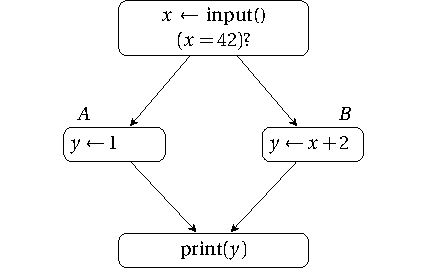
\includegraphics[scale=0.7]{ifthenelse-nonssa.pdf}\goto{CFG}{CFG}
% \hyperlink{CFG}{\beamergotobutton{?`CFG?}}
\end{minipage}

~\vspace{3cm}
%
\onslide<+->
\hskip1cm
\begin{minipage}{0.4\textwidth}
  \begin{center}
% \footnotesize
\begin{lstlisting}
  $x$ = input();
  if ($x$ == 42) {
    $y_1$ = 1;
  } else {
    $y_2$ = $x$ + 2;
  }
  $y_3$ = $\phi$($y_1$,$y_2$);
  print($y_3$);
\end{lstlisting}
  \end{center}
\end{minipage}
\begin{minipage}{0.4\textwidth}
\strut
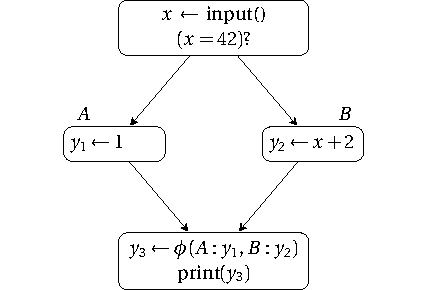
\includegraphics[scale=0.7]{ifthenelse-ssa.pdf}
\end{minipage}
\end{overprint}


\end{frame}

\begin{frame}
\frametitle{Informal Semantics}
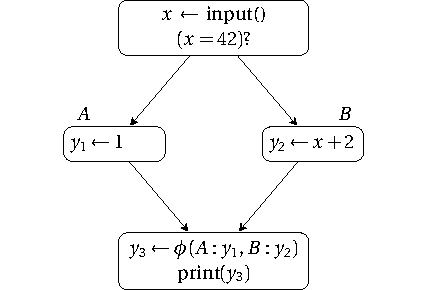
\includegraphics[scale=0.7]{ifthenelse-ssa.pdf}
\begin{minipage}[b]{0.5\textwidth}
  Introduction of $\phi$-functions:
\begin{itemize}
\item to fix the ambiguity; introduces $y_3$ which takes either $y_1$ or $y_2$
\item placed at control-flow merge points i.e., head of basic-blocks that have multiple predecessors
\end{itemize}
\vskip5mm
\end{minipage}
\begin{itemize}
\item $n$ parameters if it has $n$ incoming CFG paths
% \item optionaly can be represented as $a_0=\phi(B_1:a_1, \dots, B_n:a_n)$
\item represented as $a_0=\phi(a_1, \dots, a_n)$
\end{itemize}
\end{frame}


\begin{frame}
  \frametitle{Questions on SSA}
  $\approx$ 5 min to answer the following questions:
  \begin{exampleblock}{}
    Is it possible to have more than one $\phi$-function in a basic block?
  \end{exampleblock}
  \begin{exampleblock}{}
    How can you execute code containing $\phi$-functions on a machine?
  \end{exampleblock}

\end{frame}

\begin{frame}
\frametitle{Informal Semantics}
\begin{itemize}
\item multiple $\phi$-functions executed simultaneously:\\ 
$
\begin{array}{l}
  a=\phi(a,b)\\
  b=\phi(b,a)
\end{array}
$
\item $\phi$-functions not directly executable (IR only: for static analysis)
\item $\phi$-functions removed before assembly code generation\\
  \handr copy instructions insertion
  \pause
\item exists extensions of $\phi$-functions (e.g., $\phi_{\textrm{if}}$, $\gamma$, etc.) that take an additional predicate parameter
\end{itemize}
\end{frame}

\begin{frame}[fragile]
\frametitle{Informal Semantic}
\begin{minipage}[b]{\textwidth}
\begin{itemize}
\item SSA is not Dynamic Single Assignment (DSA or SA)
\item Construction: insert $\phi$-function where multiple reaching defs converge; version variables $x$ and $y$ (integer subscripts); 
\end{itemize}
\end{minipage}

\strut\hfill
\begin{minipage}[t]{0.3\textwidth}
  \begin{lstlisting}
  $x$ = 0;
  $y$ = 0;
  while ($x$<10) {
    $y$ = $y$ + $x$;
    $x$ = $x$ + 1;
  }
  print ($y$);
  \end{lstlisting}
\end{minipage}
\hfill
\begin{minipage}[t]{0.3\textwidth}
\strut
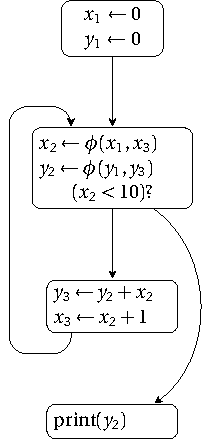
\includegraphics[valign=t,scale=0.65]{while}
\end{minipage}
\hfill\strut
\end{frame}

\begin{frame}
\frametitle{Comparison with Classical Data Flow Analysis}
\begin{itemize}
\item During actual program execution, information flows between variables
\item Static analysis captures this behavior by propagating abstract information along CFG
\item Can be propagated more efficiently using a functional or sparse representation such as SSA
\item Constant propagation: definitions $\equiv$ set of points where information may change; associate information with variable names rather than variables $\times$ program points
%- other data flow problems can be accomodated by inserting additional pseudo-definition functions at appropriate points to induice renaming
\end{itemize}
\end{frame}

\begin{frame}
\frametitle{Comparison with Classical Data Flow Analysis}
\begin{block}{Null pointer analysis}
  \begin{overprint}
    \onslide<+>
    Determine statically if variable can contain null value at run-time.
    \onslide<+->
    \begin{center}
      \footnotesize
      \begin{tabular}[t]{c@{\hskip1cm}c}
      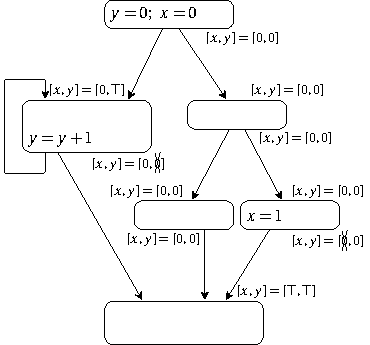
\includegraphics[valign=t,scale=0.7]{zero-1} &
      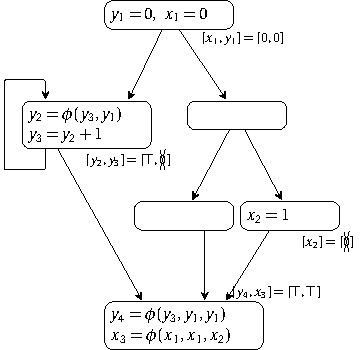
\includegraphics[valign=t,scale=0.7]{zero-2}\\[1ex]
      dense & SSA based
    \end{tabular}
    \end{center}
  \end{overprint}
\end{block}

\uncover<+->{
\begin{itemize}
\item Propagates from defs to uses (via def-use links); avoid program points where information does not change or not relevant
\item Results are more compact
\end{itemize}
}
\end{frame}

\begin{frame}
\frametitle{SSA in Context}
\begin{itemize} 
\item 1980s developments of IRs to encapsulate data dependences to expose direct link between definitions and uses (def-use chains). eg PDG, PD-web... SSA developed at IBM and published late 80s
\item GCC, Open64, HotSpot, Jikes, V8, Mono, LLVM... use SSA
\item more and more popular for JIT compilation on Java byte-code, CLI byte-code, LLVM bitcode...
\item because of favorable properties (simplification and reduced complexity) recently adopted back-end level even register allocation phase
\item also for high-level language impose referential transparency e.g. SISAL; on a per-variable basis final in Java, const or readonly in C\#. Immutability simplifies concurrent programming  
\end{itemize}
\end{frame}

\begin{frame}
\frametitle{Benefits of SSA}
\begin{itemize}
\item Compile time benefit (e.g., sparse data flow analysis)
\item Compiler development benefit (e.g., dead-code in GCC 4.x 40\% of GCC 3.x)
\item Program run-time benefit (simpler to develop more efficient analysis)
\end{itemize}
\begin{center}
\small
\begin{tabular}{p{0.45\textwidth}@{\kern.1\textwidth}p{0.43\textwidth}}
  \hfil Myth\hfil & \hfil Reality \hfil \\[1ex] \hline \\[-2ex]
Greatly increases number of vars & $\approx$10\% expansion\\ [1ex]
Destruction generates many copy ops & not more than original prog. \\ [1ex]
SSA property difficult to maintain & $\equiv$ SSA construction restricted to some variables / code region 
\end{tabular}
\end{center}
\end{frame}




%%%%%%%%%%%%%%%%%%%%%%%%%%%%%%%%%%%%%%%%%%%%%%%%%%%%%%
%%%%%%%%%%%%%%%%%%%%%%%%%%%%%%%%%%%%%%%%%%%%%%%%%%%%%%

\section{Properties and Flavors (P. Brisk, F. Rastello)}
\begin{frame}
\frametitle{Def-Use and Use-Def Chains}
\begin{itemize}
\item Def-Use chains: for a definition the set of all its uses
\item Use-Def chain: for a use the (unique under SSA) definition that reaches the use
\item direct connections to propagate data-flow information
\end{itemize}
\begin{minipage}[t]{0.5\textwidth}
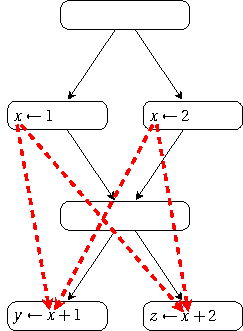
\includegraphics[valign=t,scale=0.65]{du-1}\hfill
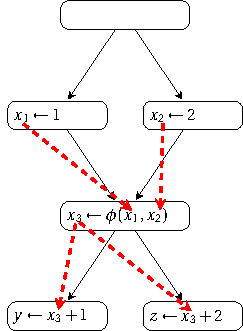
\includegraphics[valign=t,scale=0.65]{du-2}
\end{minipage}
\begin{minipage}[t]{0.48\textwidth}
\begin{itemize}
\item Information is combined as early as possible
\item Use-Def Chains for free; Def-Use Chains almost for free. 
\end{itemize}
\end{minipage}
\end{frame}

\begin{frame}
\frametitle{Minimality}
\begin{itemize}
\item Construction: place $\phi$-functions (e.g., $a=\phi(a,a)$); rename variables. Minimality is a property of the code \emph{before renaming}.
\item \emph{Single reaching-definition property}: no program point can be reached
by two definitions of the same variable
\item \emph{Minimality property}: minimality of the number of inserted $\phi$-functions
\item $n_3$ is a \emph{join node}  of $n_1$ and $n_2$ ($n_3\in {\cal J}(n_1,n_2)$) if $\exists$ two non-empty path (at least one edge), from $n_1$ to $n_3$ and from $n_2$ to $n_3$. 
\item \emph{necessary}: place $\phi$-functions of var $v$ at ${\cal J}(\textrm{Defs}_v)$
\item \emph{sufficient}: ${\cal J}(S \cup{\cal J}(S))={\cal J}(S)$
\item \emph{strictness}: in practice place at   ${\cal J}(\textrm{Defs}_v\cup r)$ 
\end{itemize}
\begin{minipage}{0.7\textwidth}
\begin{alertblock}{}
Minimality \emph{not} a requirement. Copy-propagation is enough.
\end{alertblock}
\end{minipage}
\end{frame}

\begin{frame}
\frametitle{Strict SSA Form and Dominance Property}
\begin{itemize}
\item \emph{strict}: if every variable is defined before it is used. Java imposes strictness, C++ does not.
\item $n_1$ \emph{dominates} basic block $n_2$ if every path
from $r$ to $n_2$ includes $n_1$
\end{itemize}
\begin{minipage}[t]{0.5\textwidth}
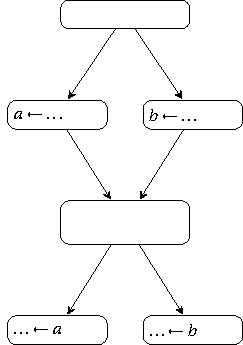
\includegraphics[valign=t,scale=0.65]{double-diamond-1}\hfill
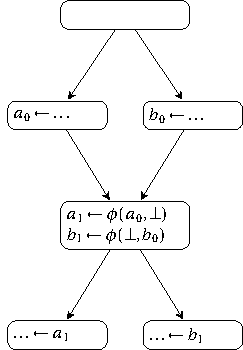
\includegraphics[valign=t,scale=0.65]{double-diamond-2}
\end{minipage}
\begin{minipage}[t]{0.45\textwidth}
\begin{itemize}
\item \emph{dominance property}: each use of a variable is dominated
by its definition
\item Add (undefined) pseudo-definition of each variable at $r$
\end{itemize}
\hspace{1cm}\goto{DomTree}{Dominator Tree}{2.5cm}
\end{minipage}
\end{frame}

\begin{frame}
\frametitle{Strict SSA Form and Dominance Property}
\begin{itemize}
\item So called ``\emph{Minimal SSA}'' (minimality and dominance property) can be efficiently built using formalism of \emph{dominance frontier} (${\cal J}(\textrm{Def}_v,r)=\textrm{DF}^+(v)$)
\item Structural properties of variables' live-range: sub-tree of the dominator tree ~~\goto{chordal}{Chordal}{1.4cm}
\begin{enumerate}
\item Fast liveness-check and iteration free liveness-set
\item Graph Coloring in linear time using \emph{tree scan} (register allocation)
\goto{spilltest}{Tree scan}{1.6cm}\end{enumerate}
\item \emph{break strictness}: e.g. copy-propagation
\item \emph{make it strict}: use standard incremental update
\end{itemize}
\begin{minipage}{0.5\textwidth}
\begin{alertblock}{}
Strictness is good especially for JIT
\end{alertblock}
\end{minipage}
\end{frame}

\begin{frame}
\frametitle{Pruned SSA Form}
\begin{itemize}
\item \emph{Minimal SSA}: $\phi$-functions where var not live prior to SSA construction
\end{itemize}
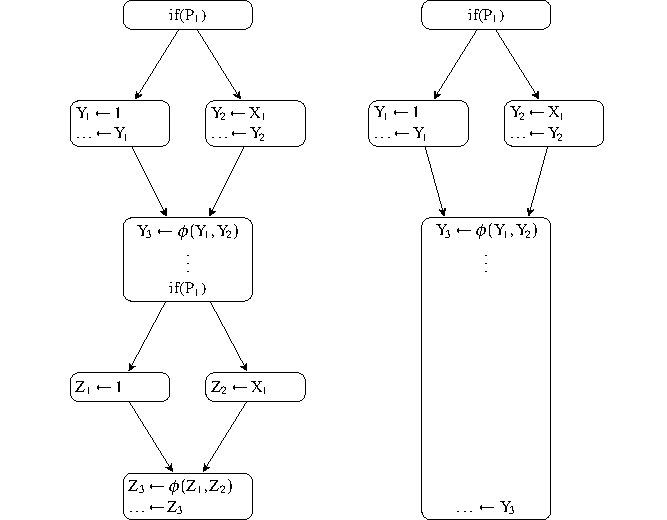
\includegraphics[valign=t,scale=0.63]{pruned}
\hspace{-0.8cm}\begin{minipage}[t]{0.47\textwidth}
\begin{itemize}
\item \emph{bad} for register allocation\\ \emph{good} for value numbering
\item \emph{pruned SSA}: without non-live $\phi$-functions
\item \emph{make it pruned}: dead-code elimination
\end{itemize}
\begin{alertblock}{}
Prune it (semi-pruned is ok) unless you \emph{really} need it
\end{alertblock}
\end{minipage}
\end{frame}

\begin{frame}
\frametitle{Conventional and Transformed SSA Form}
\begin{itemize}
\item \emph{register web}: maximum unions of def-use chains
\item \emph{$\phi$-webs}: transitive closure of $\phi$-related variables 
\end{itemize}
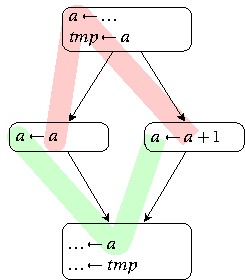
\includegraphics[valign=t,width=0.25\textwidth]{web-1}\hfill
\uncover<2->{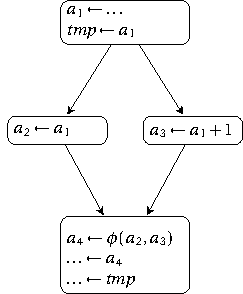
\includegraphics[valign=t,width=0.25\textwidth]{web-2}}\hfill
\uncover<3>{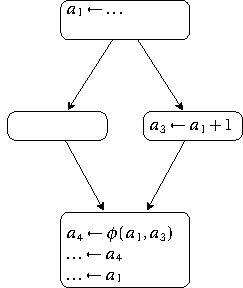
\includegraphics[valign=t,width=0.25\textwidth]{web-3}}
\begin{itemize}
\item<2-> \emph{Conventional SSA (C-SSA)}: each $\phi$-web is interference free. 
\item<3> \emph{Transformed SSA (T-SSA)}: non-conventional SSA
\end{itemize}
\end{frame}

\begin{frame}
\frametitle{Conventional and Transformed SSA Form}
\begin{itemize}
\item \emph{freshly constructed SSA}: $\phi$-web $\equiv$ register web of original non-SSA
\item \emph{destructing C-SSA}: replace each $\phi$-web by a single variable
\item \emph{make it conventional}: as ``difficult'' as destructing SSA: insert copies to dissociate interfering vars from the connecting $\phi$-functions.
\end{itemize}
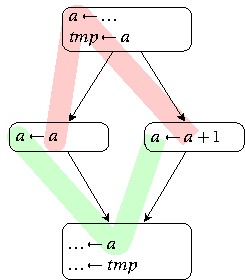
\includegraphics[valign=t,width=0.25\textwidth]{web-1}\hfill
\uncover{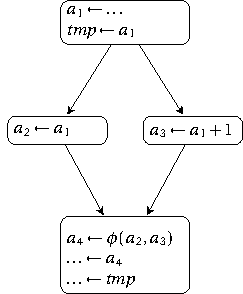
\includegraphics[valign=t,width=0.25\textwidth]{web-2}}\hfill
\uncover{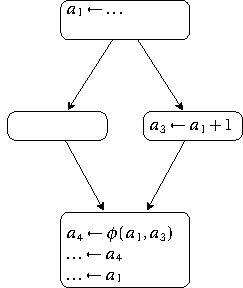
\includegraphics[valign=t,width=0.25\textwidth]{web-3}}
\begin{minipage}{0.7\textwidth}
\begin{alertblock}{}
\emph{Don't} try to enforce conventional property but for the really last phases of code generation
\end{alertblock}
\end{minipage}
\end{frame}



  
%%%%%%%%%%%%%%%%%%%%%%%%%%%%%%%%%%%%%%%%%%%%%%%%
%%%% Register allocation
%%%%%%%%%%%%%%%%%%%%%%%%%%%%%%%%%%%%%%%%%%%%%%%%
\section{Register Allocation (F. Bouchez)}

\subsection*{The rules of the game}
\begin{frame}
  \frametitle{What is register allocation?}
    \begin{block}{Assign variables (unbounded) to}
       registers (\includegraphics[width=0.12\textwidth]{registers.fig}) \& memory (infinite)
    \end{block}
   \begin{block}{Architectural subtleties}
        Specific registers (sp, fp, r0), variable affinities (auto-inc), register pairing (64 bits
          ops), distributed register banks, etc.
    \end{block}
   \begin{minipage}{0.7\textwidth}
    \begin{block}{Rules of the game}
      \begin{itemize}
        \item Fixed instruction schedule
        \item \alert{Spill}: insert {\sc loads} and {\sc stores}
        \item \alert{Coalesce}: delete {\sc moves}
        \item \alert{Split}: add register-to-register {\sc moves}
      \end{itemize}
    \end{block}
   \end{minipage}
\end{frame}

\begin{frame}
  \frametitle{What is register allocation (cont'd)?}
  \begin{block}{Allocation versus assignment}
    \begin{itemize}
      \item Allocation: which variables are allocated to memory (spilled), which ones are allocated to registers?
      \item Assignment: assign non spilled variables to registers
    \end{itemize}
  \end{block}
  \begin{block}{Allocation problem}
    \begin{itemize}
      \item \alert<3>{The spill test:} is spilling necessary (assignment feasible)?
      \item \alert<2>{What to spill and where to insert loads \& stores?}
    \end{itemize}
  \end{block}
\end{frame}

\begin{frame}
\frametitle{In-Two-Phases Register Allocation and Tree-Scan}

\only<1>{\tikzstyle{spilltest} = [concept]}
\only<2->{\tikzstyle{spilltest} = [concept]}
\only<1>{\tikzstyle{liverangesplitting} = [concept, opacity=0]}
\only<2->{\tikzstyle{liverangesplitting} = [concept]}
\only<1-2>{\tikzstyle{twophases} = [concept, opacity=0]}
\only<3->{\tikzstyle{twophases} = [concept]}
\only<1-3>{\tikzstyle{treescan} = [concept, opacity=0]}
\only<4->{\tikzstyle{treescan} = [concept]}
\only<1-3>{\tikzstyle{SSAproperties} = [concept, opacity=0]}
\only<4->{\tikzstyle{SSAproperties} = [concept]}
\tikzstyle{child6} = [concept color=blue,opacity=0]
\tikzstyle{child7} = [concept color=blue,opacity=0]
\tikzset{mybox/.style = {rectangle, minimum width=0pt, minimum height=0pt, text
    = black, font = \small}}

\begin{tikzpicture}[transform shape,scale=0.9]
    \path[mindmap,concept color=black,text=white]
    node[spilltest, scale=0.7] (SPILL) at (0,-3.5) {
      {\bf Spill test:}\\
      \only<1>{(NP-complete?}
      \only<2->{$r$-colorable\\ $\Longleftrightarrow$\\ $\textrm{MAXLIVE}\leq r$} 
    }

    child[liverangesplitting, grow=90, level distance=100] { node[concept, scale=0.7] (SPLIT) {Live-range splitting} }

    node[twophases, scale=0.7] (TWO) at (4,-4.5) {Two-phases reg-alloc\\ Simpler/better}
    node[treescan, scale=0.7] (TREESCAN) at (9,-5) {Tree-scan\\ Faster/less memory}
    child[SSAproperties, grow=120, level distance=160] { node[concept, scale=0.7] (SSA)  {SSA properties} };

    \draw<3-> [circle connection bar] (SPILL) edge (TWO);
    \draw<4-> [circle connection bar] (TWO) edge (TREESCAN);
\end{tikzpicture}

\begin{block}{}
  \only<1>{Chaitin's reduction proves the NP-completeness of the spill test...}%
  \only<2>{...under the assumption that live-range splitting is not possible.}%
  \only<3>{Spill test should not be coupled to global coloration anymore}%
  \only<4>{Tree-shaped SSA live-ranges allows for tree-based allocation schemes} 

\end{block}
\end{frame}

\subsection*{How SSA simplifies register allocation}

%BB
\begin{frame}
  \frametitle{``Spilling easier on a BB than on a general CFG''}
    \begin{columns}
    \column{0.3\textwidth}{%BB large
      \begin{center}
	\blue{Basic block}\\
	\only<1>{\includegraphics[height=5cm]{code_BB-1.fig}}%
	\only<2>{\includegraphics[height=5cm]{code_BB-2.fig}}%
	\only<3>{\includegraphics[height=5cm]{code_BB-3.fig}}%
	\only<4>{\includegraphics[height=5cm]{code_BB-4.fig}}%
	\only<5>{\includegraphics[height=5cm]{code_BB-5.fig}}%
	\only<6>{\includegraphics[height=5cm]{code_BB-6.fig}}%
	\only<7>{\includegraphics[height=5cm]{code_BB-7.fig}}%
	\only<8>{\includegraphics[height=5cm]{code_BB-8.fig}}%
	\only<9>{\includegraphics[height=5cm]{code_BB-9.fig}}%
	\only<10>{\includegraphics[height=5cm]{code_BB-10.fig}}%
	\only<11>{\includegraphics[height=5cm]{code_BB-11.fig}}%
	\only<12>{\includegraphics[height=5cm]{code_BB-12.fig}}%
	\only<13>{\includegraphics[height=5cm]{code_BB-13.fig}}%
	\only<14>{\includegraphics[height=5cm]{code_BB-14.fig}}%
	\begin{block}{}
	  \begin{itemize}
	  \item $\textsf{MAXLIVE}\leq r$
	  \item Linear scan
	  \end{itemize}
	\end{block}
      \end{center}
    }
    \column{0.3\textwidth}{%SSA small
      \begin{center}
	\blue{SSA code}\\
	\includegraphics[height=2.5cm]{code_SSA-1.fig}%
      \end{center}
    }
    \column{0.3\textwidth}{%CFG small
      \begin{center}
	\blue{General CFG}\\
	\includegraphics[height=2.5cm]{code_CFG-1.fig}    
      \end{center}
    }
    \end{columns}
\end{frame}
 
%CFG
\begin{frame}
  \frametitle{``Spilling easier on a BB than on a general CFG''}
  \begin{columns}
    \column{0.15\textwidth}{%BB
      \begin{center}
	\blue{BB}\\
	\includegraphics[height=2.5cm]{code_BB-8.fig}
      \end{center}
    }
    \column{0.15\textwidth}{%SSA small
       \begin{center}
	 \blue{SSA}\\
	 \includegraphics[height=2.5cm]{code_SSA-1.fig}%
       \end{center}
    }
    \column{0.45\textwidth}{%CFG
      \begin{center}
	\blue{General control flow graph}\\
	\includegraphics[height=5cm]{code_CFG_static.fig}    
	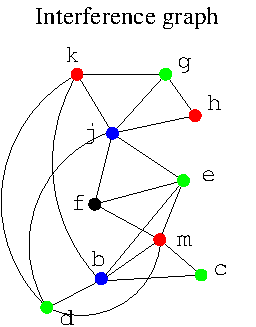
\includegraphics[height=3cm]{IntGraph-stuck.fig}  
	\begin{alertblock}{}
	  \begin{itemize}
	  \item Coloring test
	  \item Greedy coloring
	  \end{itemize}
	\end{alertblock}
      \end{center}
   }%
  \end{columns}
\end{frame}

%SSA
\begin{frame}
  \frametitle{``Under SSA: the dominance tree''}
    \begin{columns}
    \column{0.15\textwidth}{%
      \begin{center}
	\blue{BB}\\
	\includegraphics[height=2.5cm]{code_BB-8.fig}
      \end{center}
    }
    \column{0.55\textwidth}{%
      \begin{center}
	\blue{Static single assignment form}\\
	\only<1>{\includegraphics[height=5cm]{code_SSA-1.fig}}%
	\only<2>{\includegraphics[height=5cm]{code_SSA-2.fig}}%
	\only<3>{\includegraphics[height=5cm]{code_SSA-3.fig}}%
	\only<4>{\includegraphics[height=5cm]{code_SSA-4.fig}}%
	\only<5>{\includegraphics[height=5cm]{code_SSA-5.fig}}%
	\only<6>{\includegraphics[height=5cm]{code_SSA-6.fig}}%
	\only<7>{\includegraphics[height=5cm]{code_SSA-7.fig}}%
	\only<8>{\includegraphics[height=5cm]{code_SSA-8.fig}}%
	\only<9>{\includegraphics[height=5cm]{code_SSA-9.fig}}%
	\only<10>{\includegraphics[height=5cm]{code_SSA-10.fig}}%
	\only<11>{\includegraphics[height=5cm]{code_SSA-11.fig}}%
	\only<12>{\includegraphics[height=5cm]{code_SSA-12.fig}}%
	\only<13>{\includegraphics[height=5cm]{code_SSA-13.fig}}%
	\only<14>{\includegraphics[height=5cm]{code_SSA-14.fig}}%
	\begin{block}{}
	  \begin{itemize}
	  \item $\textsf{MAXLIVE}\leq r$
	  \item Tree scan
	  \end{itemize}
	\end{block}
      \end{center}
    }%
    \column{0.3\textwidth}{%
      \begin{center}
      \blue{CFG}\\
      \includegraphics[height=2.5cm]{code_CFG_static.fig}    
      \includegraphics[height=1.5cm]{IntGraph.fig}  
      \end{center}
    }     
  \end{columns}
\end{frame}

\begin{frame}
  \frametitle{``Under SSA: the dominance tree''}
    \begin{columns}
    \column{0.28\textwidth}{%BB
      \blue{Basic block}\\
      \includegraphics[height=3.5cm]{code_BB-8.fig}
      \begin{block}{}
	\begin{itemize}
	  \item $\textsf{MAXLIVE}\leq r$
	  \item Linear scan
	\end{itemize}
      \end{block}
    }
    \column{0.28\textwidth}{%SSA
      \blue{SSA form}\\
      \includegraphics[height=3.5cm]{code_SSA-8.fig}%
    \begin{block}{}
	 \begin{itemize}
	 \item $\textsf{MAXLIVE}\leq r$
	 \item Tree scan
	 \end{itemize}
      \end{block}
    }%
    \column{0.35\textwidth}{%CFG
      \blue{General CFG}\\
      \includegraphics[height=3.5cm]{code_CFG_static.fig}    
      \includegraphics[height=2cm]{IntGraph.fig}  
      \begin{alertblock}{}
	\begin{itemize}
	\item Coloring test
	\item Greedy coloring
	\end{itemize}
      \end{alertblock}
    }     
  \end{columns}
\end{frame}

\begin{frame}
  \frametitle{Why coalescing?}
  \begin{block}{Goal of coalescing}
    Removing the register-to-register copies [\texttt{move $a \gets b$}]
  \end{block}
   \begin{columns}
    \column{.38\textwidth}{
    Numerous copies due to:
    \smallskip
  \begin{itemize}[<+-| alert@+>]
    \item live-range splitting to avoid spilling % in particual, reg alloc in 2 phases
    \item register constraints
    \item \alert<.-.(1)>{SSA destruction}
  \end{itemize}
  \vfill
~
\vspace{6em}\\
  }%
 \hfill
 \setcounter{beamerpauses}{2}
  \column{.6\textwidth}{%
  \centering%
%  \begin{example}<+->%
  \only<+->{
  \begin{exampleblock}{}
    \only<-.>{%
    \tikzfigure{move-reg-constr}%
    }%
    \only<+->{%
    \vspace{-4mm}
    \tikzfigure{move-out-SSA}%
    }%
%  \end{example}%
  \end{exampleblock}%
  }%
 }
 \end{columns}%
\end{frame}

\subsubsection*{What is new?}

% Let us summaries what I have understood. With enough live-range splitting, there is no need to
% spill more than lowering MAXLIVE to the number of available registers. SSA based splitting do the job.
% But these ideas are not new!
\begin{frame}[label=past]
\frametitle{The past}
Live-range splitting already considered in the past:
\begin{itemize}
\item \emph{\textsf{MAXLIVE} registers are sufficient if aggressive splitting is performed}: already pointed out by Fabri, and Cytron \& Ferrante (but did not mention the possible need of critical edge splitting).
 \item Briggs tried SSA-based splitting (PhD thesis)
\end{itemize}
\uncover<2->{
But,
\begin{itemize}
 \item[\sad] These ideas were not exploited (coalescing not good enough?)
 \item[\red{\txtimpl}] Instead: sophisticated algorithms that split on demand
when the coloring fails, e.g., live-range splitting (Cooper and
Simpson), optimistic (Park and
Moon), priority based (Chow and
Hennessy, etc.
\end{itemize}}
\end{frame}

\begin{frame}[label=past]
  \frametitle{The present}
\includegraphics[width=\textwidth]{scheme_anim-4.fig}
  \begin{itemize}
  \item[1.] \alert{Spill} so as to lower register pressure to $\leq$ \#registers
  \item \alert{Split} so that interference graph is \gr{k} 
    ( $\sim$ $k$-colorable {\it \`a la} Chaitin)
  \item[2.] \alert{Color + Coalesce} to remove useless copies
  \end{itemize}

\begin{alertblock}{Exploit Greedy-$k$-colorable graph properties}
SSA based live-range splitting leads to an interference graph that can be $k$-colored ($k = \textsf{MAXLIVE}$) using Chaitin's simplification scheme. 
\end{alertblock}

\begin{alertblock}{Optimize coalescing separately from spilling}
\end{alertblock}
\end{frame}



\subsection*{Important notions}


\subsubsection*{Aggressive versus conservative coalescing}
\begin{frame}[label=past]
  \only<1-3>{\frametitle{Aggressive coalescing}}
  \only<4->{\frametitle{Conservative coalescing}}
   \alert<1-3>{Aggressive}
  coalescing may lead to spilling. \alert<4>{Conservative} coalescing
  takes colorability into account.  

\vfill
  \begin{center}    \begin{tikzpicture}[scale=1.1, auto,swap]
\small

      % a simple graph
      \node[vertex] (b) at (1,1) {\only<-3>{b}\only<4>{\red{b}}} ;
      \node[vertex] (c) at (1,0) {c} ;
      \node[vertex] (a) at (0,1) {\only<2-3>{\red{a}}\only<1,4>{a}} ;
      \node[vertex] (d) at (0,0) {\only<1>{d}\only<2->{\red{d}}} ;
      \path[interf] (b) -- (c) ;
      \path[interf] (a) -- (b) ;
      \path[interf] (c) -- (d) ;
      \path[affinity] (a) -- (d) ;
      \path[affinity] (b) -- (d) ;

      \path node at (0,-1) {} ;

      \path<3-> node[draw,anchor=south west] at (0,-1) {2-colorable} ;

      % une petite fleche
      \draw[->,thick, double] (1.5,1.5) .. controls (2,2) and (3,2) .. (3.5,1.5) ;
      % avec du texte
      \path<-3> node[draw,anchor=south] at (2.5,2) {Coalesce aggressively} ;
      \path<4-> node[draw,anchor=south] at (2.5,2) {Coalesce conservatively} ;

      % on decale la suite vers la droite
      \begin{scope}[xshift=4cm]
        % invisible node so that it doesn't move when changing slides
        \path node at (1.3,1) {} ;

        % les memes qui n'ont pas bouge
        \path<2-> node[vertex] (b) at (1,1) {b} ;
        \path<2-> node[vertex] (c) at (1,0) {c} ;
        \path[interf]<2-> (c) -- (b) ;

        % coalescing de a et d
        \path[vertex]<2-3> node[vertex] (ad) at (0,0.5) {\red{ad}} ;
        \path[interf]<2-3> (ad) -- (b) ;
        \path[interf]<2-3> (ad) -- (c) ;
        \path[affinity]<2-3> (b) .. controls (0.45,1) .. (ad) ;

        \path<3> node[draw, anchor=south east,red] at (1,-1) {Not 2-colorable};

        % coalescing de b et d
        \path<4> node[vertex] (a) at (0,1) {a} ;
        \path<4> node[vertex](bd) at (1,1) {\red{bd}} ;
        \path[interf]<4> (a) -- (bd) ;
        \path[affinity]<4> (a) .. controls (0.4,0.7) and (0.6,0.7) .. (bd) ;

        \path<4> node[draw, anchor=south east,green] at (1,-1) {2-colorable} ;
      \end{scope}

    \end{tikzpicture}


\end{center}
\end{frame}

\subsubsection*{\Gr{k} graphs}
\begin{frame}[label=past]
  \frametitle{\Gr{k} graphs}
\vspace{-2cm}
$k$-colorability is hard to check, but
\alert{greedy-k-colorability} is easy.
  \begin{block}{}
  Check greedy-$k$-colorability: simplify nodes with $<k$ neighbors.% {\it ($k=3$)}
  \end{block}
  \vfill

%  \begin{overprint}
%  \begin{overlayarea}{\textwidth}{3cm}
%    \setcounter{tmp}{0}

  \def\simplifylist{0,10,9,7,6,13,5,4,12,2,3,1,11}
  \def\coloringlist{11,1,3,2,12,4,5,13,6,7,9,10,0}
%  \def\simplifylist{0,10,9,7}
%  \def\coloringlist{9,10,0}

  \printaffinitystatusfalse

  \simplifyingtrue
  \foreach \simplifyme in \simplifylist {
    \only<+>{\begin{tikzpicture}[overlay,shift={(current page.south west)}]

\ifx\inktikz\undefined
\else
%\begin{tikzpicture}
%\newif\ifsimplifying
%\simplifyingtrue
%\newif\ifprintaffinitystatus
%\printaffinitystatusfalse
  \def\nodelist{0,1,11,10,9,7,13,6,12,5,4,2,3}
  \def\simplifyme{9}
\fi


\begin{scope}[shift={(3cm,1cm)}]


\tikzstyle{normal interf} = [draw, black, thick]
\tikzstyle{simplified interf} = [draw, gray!30, thick]

\tikzstyle{affinity} = [dashed]

\tikzstyle{normal vertex} = [vertex]
\tikzstyle{simplified vertex} = [vsimpl]


  \countdef\counters=10

  \advance\counters by 1
  \countdef\returnvalue=\the\counters  % count for return value of functions

  \xdef\nodestatus{\the\counters} %nodestatus + node number
  \count1=\the\counters
  \advance\count1 by 20 
  \xdef\nodedegree{\the\count1} %nodestatus + node number

%  \message{Node status are from \nodestatus and degree from \nodedegree}

  \def\getanyval#1-#2.{{
    \count1=#1
    \advance\count1 by #2
    \global\returnvalue=\the\count\the\count1%
%    \message{Regs #1: got value of r#2 (i.e, reg {\the\count1}): it is \the\count\the\count1 (\the\returnvalue)}
  }}

  \def\setanyval#1-#2.#3{{
    \count1=#1
    \advance\count1 by #2%
    \global\count\the\count1=#3
  %  \message{Regs #1: set r#2 to #3 (i.e, reg {\the\count1} to \the\count\the\count1)}
  }}


  \def\getval#1{\getanyval\nodestatus-#1.}
  \def\setval#1.#2{\setanyval\nodestatus-#1.{#2}}

  \def\incrdegree#1{{
    \count1=\nodedegree
    \advance\count1 by #1
    \global\advance\count\the\count1 by 1
  }}

  \def\getdegree#1{\getanyval\nodedegree-#1.}


  \newif\ifsimplified

  \def\testedge#1-#2{
  \getval{#1}
    \ifnum\the\returnvalue=0
    \getval{#2}
      \ifnum\the\returnvalue=0
%        \message{NORMAL edge #1-#2}
        \simplifiedfalse
        \def\estyle{normal interf}
     \else
%       \message{SIMPLIFIED edge#1-#2}
       \simplifiedtrue
       \def\estyle{simplified interf}
     \fi
   \else
%     \message{SIMPLIFIED edge#1-#2}
     \simplifiedtrue
     \def\estyle{simplified interf}
   \fi
  }

  \def\testnode#1,#2.#3{%
    \getval{#1}%
    \ifnum\the\returnvalue=0
      \ifsimplifying
        \def\nstyle{normal vertex}
      \else
        \def\nstyle{vert#3}
      \fi
    \else
      \def\nstyle{simplified vertex}
%      \message{#1 (#2) seems to be simplified}
      \node at (stack#1) {$#2$};
    \fi
  }

  \def\newnode#1-#2-(#3)#4{
    \testnode#1,#2.#4
    \node[\nstyle] (n#1) at (#3) {$#2$};
  }

  \def\newedge#1-#2{
    \testedge{#1}-{#2}
    \ifsimplified\else
      \incrdegree{#1}
      \incrdegree{#2}
    \fi
    \path[\estyle] (n#1) -- (n#2);
  }

  \def\newaff#1-#2#3{
    \testedge{#1}-{#2}
    \ifprintaffinitystatus
      \path[affinity#3] (n#1) -- (n#2);
    \else\fi
    \path[\estyle,affinity] (n#1) -- (n#2);
  }


  \path (-1.8,-3.9) coordinate (stack top)
  ++(-2em,2.8) node[rotate=90] {{\sl Stack}};

  \def\stackheight{4.8}
  \draw[rounded corners=1mm] (stack top) ++(0,.5cm) -- ++(-1em,0) -- +(0,\stackheight) -- +(0,0) -- ++(2em,0) -- +(0,\stackheight);

  \def\addtostack#1{
%  \node[above=1ex of stack top,name=stack#1] (stack top) {};
    \node[above=.6em of stack top] (stack#1) {};
    \coordinate (stack top) at (stack#1);
%  \message{#1 put on stack}
  }
  

  \def\dosimplify#1{
  \foreach \x in \nodelist {
    \setval\x.1
    \addtostack{\x}
    \ifnum\x=#1
      \breakforeach
    \else
    \fi
  }}

  \foreach \x in \nodelist {
    \setval\x.0 ;
    \setanyval\nodedegree-\x.0 ;
  }
  \dosimplify{\simplifyme}

  \foreach \x in \nodelist {
    \getval\x
%    \message{***************************** \x  is \ifnum\the\returnvalue=0 normal\else simplified\fi}
  }

  \begin{scope}[scale=1.2,yshift=.5cm,xshift=-.5cm]

  \newnode1-a-(1,0)r
  \newnode2-b-(2,-2)g
  \newnode3-c-(1,-2)b
  \newnode4-d-(3,-1)r
  \newnode5-e-(4,-1)g
  \newnode6-f-(5,-1)r
  \newnode7-g-(6,-2)g

  \newnode9-i-(6,-1)b
  \newnode10-j-(7,0)g

  \newnode11-c'-(0,-2)g
  \newnode12-d'-(2,-1)r
  \newnode13-g'-(4,-2)b

  \newedge1-3
  \newedge1-2
  \newedge1-{11}
  \newedge2-4
  \newedge2-3
  \newedge2-{12}
  \newedge3-4
  \newedge3-{12}
  \newedge4-5
  \newedge5-6
  \newedge5-{13}
  \newedge6-7
  \newedge6-9
  \newedge6-{13}
  \newedge7-9
  \newedge9-{10}


  \newaff3-{11}r
  \newaff4-{12}g
  \newaff7-{13}r
  \newaff1-{10}r
\end{scope}

  % Now print the degree
  \ifsimplifying
  \foreach \x in \nodelist {
    \getdegree{\x}
%    \message{degree of \x is \the\returnvalue}
    \ifnum\the\returnvalue>0
    \adddegree\the\returnvalue to n\x.
    \else
    \fi

    %legend
	}
	{%[scale=.5,every node/.style={transform shape}]
	\it
	\scriptsize
    \node[degree label={red!80!magenta},right,transform shape,minimum size=1.5ex] (x) at (0,-2.8)  {} ;
	\node[right=1ex of x] {Hi-degree node};
    \node[degree label=green!80!blue,below=1ex of x,minimum size=1.5ex] (x) {};
	\node[right=1ex of x] {Low-degree node};
	}
  \else\fi



%\useasboundingbox (-2.1,-3.5) rectangle ++ (9.5,5.5);
%\dbbox


\end{scope}
\end{tikzpicture}
%
    \message{Simplifing \simplifyme}
    }
  }

  \simplifyingfalse
  \foreach \simplifyme in \coloringlist {
    \only<+>{\begin{tikzpicture}[overlay,shift={(current page.south west)}]

\ifx\inktikz\undefined
\else
%\begin{tikzpicture}
%\newif\ifsimplifying
%\simplifyingtrue
%\newif\ifprintaffinitystatus
%\printaffinitystatusfalse
  \def\nodelist{0,1,11,10,9,7,13,6,12,5,4,2,3}
  \def\simplifyme{9}
\fi


\begin{scope}[shift={(3cm,1cm)}]


\tikzstyle{normal interf} = [draw, black, thick]
\tikzstyle{simplified interf} = [draw, gray!30, thick]

\tikzstyle{affinity} = [dashed]

\tikzstyle{normal vertex} = [vertex]
\tikzstyle{simplified vertex} = [vsimpl]


  \countdef\counters=10

  \advance\counters by 1
  \countdef\returnvalue=\the\counters  % count for return value of functions

  \xdef\nodestatus{\the\counters} %nodestatus + node number
  \count1=\the\counters
  \advance\count1 by 20 
  \xdef\nodedegree{\the\count1} %nodestatus + node number

%  \message{Node status are from \nodestatus and degree from \nodedegree}

  \def\getanyval#1-#2.{{
    \count1=#1
    \advance\count1 by #2
    \global\returnvalue=\the\count\the\count1%
%    \message{Regs #1: got value of r#2 (i.e, reg {\the\count1}): it is \the\count\the\count1 (\the\returnvalue)}
  }}

  \def\setanyval#1-#2.#3{{
    \count1=#1
    \advance\count1 by #2%
    \global\count\the\count1=#3
  %  \message{Regs #1: set r#2 to #3 (i.e, reg {\the\count1} to \the\count\the\count1)}
  }}


  \def\getval#1{\getanyval\nodestatus-#1.}
  \def\setval#1.#2{\setanyval\nodestatus-#1.{#2}}

  \def\incrdegree#1{{
    \count1=\nodedegree
    \advance\count1 by #1
    \global\advance\count\the\count1 by 1
  }}

  \def\getdegree#1{\getanyval\nodedegree-#1.}


  \newif\ifsimplified

  \def\testedge#1-#2{
  \getval{#1}
    \ifnum\the\returnvalue=0
    \getval{#2}
      \ifnum\the\returnvalue=0
%        \message{NORMAL edge #1-#2}
        \simplifiedfalse
        \def\estyle{normal interf}
     \else
%       \message{SIMPLIFIED edge#1-#2}
       \simplifiedtrue
       \def\estyle{simplified interf}
     \fi
   \else
%     \message{SIMPLIFIED edge#1-#2}
     \simplifiedtrue
     \def\estyle{simplified interf}
   \fi
  }

  \def\testnode#1,#2.#3{%
    \getval{#1}%
    \ifnum\the\returnvalue=0
      \ifsimplifying
        \def\nstyle{normal vertex}
      \else
        \def\nstyle{vert#3}
      \fi
    \else
      \def\nstyle{simplified vertex}
%      \message{#1 (#2) seems to be simplified}
      \node at (stack#1) {$#2$};
    \fi
  }

  \def\newnode#1-#2-(#3)#4{
    \testnode#1,#2.#4
    \node[\nstyle] (n#1) at (#3) {$#2$};
  }

  \def\newedge#1-#2{
    \testedge{#1}-{#2}
    \ifsimplified\else
      \incrdegree{#1}
      \incrdegree{#2}
    \fi
    \path[\estyle] (n#1) -- (n#2);
  }

  \def\newaff#1-#2#3{
    \testedge{#1}-{#2}
    \ifprintaffinitystatus
      \path[affinity#3] (n#1) -- (n#2);
    \else\fi
    \path[\estyle,affinity] (n#1) -- (n#2);
  }


  \path (-1.8,-3.9) coordinate (stack top)
  ++(-2em,2.8) node[rotate=90] {{\sl Stack}};

  \def\stackheight{4.8}
  \draw[rounded corners=1mm] (stack top) ++(0,.5cm) -- ++(-1em,0) -- +(0,\stackheight) -- +(0,0) -- ++(2em,0) -- +(0,\stackheight);

  \def\addtostack#1{
%  \node[above=1ex of stack top,name=stack#1] (stack top) {};
    \node[above=.6em of stack top] (stack#1) {};
    \coordinate (stack top) at (stack#1);
%  \message{#1 put on stack}
  }
  

  \def\dosimplify#1{
  \foreach \x in \nodelist {
    \setval\x.1
    \addtostack{\x}
    \ifnum\x=#1
      \breakforeach
    \else
    \fi
  }}

  \foreach \x in \nodelist {
    \setval\x.0 ;
    \setanyval\nodedegree-\x.0 ;
  }
  \dosimplify{\simplifyme}

  \foreach \x in \nodelist {
    \getval\x
%    \message{***************************** \x  is \ifnum\the\returnvalue=0 normal\else simplified\fi}
  }

  \begin{scope}[scale=1.2,yshift=.5cm,xshift=-.5cm]

  \newnode1-a-(1,0)r
  \newnode2-b-(2,-2)g
  \newnode3-c-(1,-2)b
  \newnode4-d-(3,-1)r
  \newnode5-e-(4,-1)g
  \newnode6-f-(5,-1)r
  \newnode7-g-(6,-2)g

  \newnode9-i-(6,-1)b
  \newnode10-j-(7,0)g

  \newnode11-c'-(0,-2)g
  \newnode12-d'-(2,-1)r
  \newnode13-g'-(4,-2)b

  \newedge1-3
  \newedge1-2
  \newedge1-{11}
  \newedge2-4
  \newedge2-3
  \newedge2-{12}
  \newedge3-4
  \newedge3-{12}
  \newedge4-5
  \newedge5-6
  \newedge5-{13}
  \newedge6-7
  \newedge6-9
  \newedge6-{13}
  \newedge7-9
  \newedge9-{10}


  \newaff3-{11}r
  \newaff4-{12}g
  \newaff7-{13}r
  \newaff1-{10}r
\end{scope}

  % Now print the degree
  \ifsimplifying
  \foreach \x in \nodelist {
    \getdegree{\x}
%    \message{degree of \x is \the\returnvalue}
    \ifnum\the\returnvalue>0
    \adddegree\the\returnvalue to n\x.
    \else
    \fi

    %legend
	}
	{%[scale=.5,every node/.style={transform shape}]
	\it
	\scriptsize
    \node[degree label={red!80!magenta},right,transform shape,minimum size=1.5ex] (x) at (0,-2.8)  {} ;
	\node[right=1ex of x] {Hi-degree node};
    \node[degree label=green!80!blue,below=1ex of x,minimum size=1.5ex] (x) {};
	\node[right=1ex of x] {Low-degree node};
	}
  \else\fi



%\useasboundingbox (-2.1,-3.5) rectangle ++ (9.5,5.5);
%\dbbox


\end{scope}
\end{tikzpicture}
%
    \message{Coloring \simplifyme}%
    }
  }
  {
    \printaffinitystatustrue
    \def\simplifyme{0}
    \only<+>{\begin{tikzpicture}[overlay,shift={(current page.south west)}]

\ifx\inktikz\undefined
\else
%\begin{tikzpicture}
%\newif\ifsimplifying
%\simplifyingtrue
%\newif\ifprintaffinitystatus
%\printaffinitystatusfalse
  \def\nodelist{0,1,11,10,9,7,13,6,12,5,4,2,3}
  \def\simplifyme{9}
\fi


\begin{scope}[shift={(3cm,1cm)}]


\tikzstyle{normal interf} = [draw, black, thick]
\tikzstyle{simplified interf} = [draw, gray!30, thick]

\tikzstyle{affinity} = [dashed]

\tikzstyle{normal vertex} = [vertex]
\tikzstyle{simplified vertex} = [vsimpl]


  \countdef\counters=10

  \advance\counters by 1
  \countdef\returnvalue=\the\counters  % count for return value of functions

  \xdef\nodestatus{\the\counters} %nodestatus + node number
  \count1=\the\counters
  \advance\count1 by 20 
  \xdef\nodedegree{\the\count1} %nodestatus + node number

%  \message{Node status are from \nodestatus and degree from \nodedegree}

  \def\getanyval#1-#2.{{
    \count1=#1
    \advance\count1 by #2
    \global\returnvalue=\the\count\the\count1%
%    \message{Regs #1: got value of r#2 (i.e, reg {\the\count1}): it is \the\count\the\count1 (\the\returnvalue)}
  }}

  \def\setanyval#1-#2.#3{{
    \count1=#1
    \advance\count1 by #2%
    \global\count\the\count1=#3
  %  \message{Regs #1: set r#2 to #3 (i.e, reg {\the\count1} to \the\count\the\count1)}
  }}


  \def\getval#1{\getanyval\nodestatus-#1.}
  \def\setval#1.#2{\setanyval\nodestatus-#1.{#2}}

  \def\incrdegree#1{{
    \count1=\nodedegree
    \advance\count1 by #1
    \global\advance\count\the\count1 by 1
  }}

  \def\getdegree#1{\getanyval\nodedegree-#1.}


  \newif\ifsimplified

  \def\testedge#1-#2{
  \getval{#1}
    \ifnum\the\returnvalue=0
    \getval{#2}
      \ifnum\the\returnvalue=0
%        \message{NORMAL edge #1-#2}
        \simplifiedfalse
        \def\estyle{normal interf}
     \else
%       \message{SIMPLIFIED edge#1-#2}
       \simplifiedtrue
       \def\estyle{simplified interf}
     \fi
   \else
%     \message{SIMPLIFIED edge#1-#2}
     \simplifiedtrue
     \def\estyle{simplified interf}
   \fi
  }

  \def\testnode#1,#2.#3{%
    \getval{#1}%
    \ifnum\the\returnvalue=0
      \ifsimplifying
        \def\nstyle{normal vertex}
      \else
        \def\nstyle{vert#3}
      \fi
    \else
      \def\nstyle{simplified vertex}
%      \message{#1 (#2) seems to be simplified}
      \node at (stack#1) {$#2$};
    \fi
  }

  \def\newnode#1-#2-(#3)#4{
    \testnode#1,#2.#4
    \node[\nstyle] (n#1) at (#3) {$#2$};
  }

  \def\newedge#1-#2{
    \testedge{#1}-{#2}
    \ifsimplified\else
      \incrdegree{#1}
      \incrdegree{#2}
    \fi
    \path[\estyle] (n#1) -- (n#2);
  }

  \def\newaff#1-#2#3{
    \testedge{#1}-{#2}
    \ifprintaffinitystatus
      \path[affinity#3] (n#1) -- (n#2);
    \else\fi
    \path[\estyle,affinity] (n#1) -- (n#2);
  }


  \path (-1.8,-3.9) coordinate (stack top)
  ++(-2em,2.8) node[rotate=90] {{\sl Stack}};

  \def\stackheight{4.8}
  \draw[rounded corners=1mm] (stack top) ++(0,.5cm) -- ++(-1em,0) -- +(0,\stackheight) -- +(0,0) -- ++(2em,0) -- +(0,\stackheight);

  \def\addtostack#1{
%  \node[above=1ex of stack top,name=stack#1] (stack top) {};
    \node[above=.6em of stack top] (stack#1) {};
    \coordinate (stack top) at (stack#1);
%  \message{#1 put on stack}
  }
  

  \def\dosimplify#1{
  \foreach \x in \nodelist {
    \setval\x.1
    \addtostack{\x}
    \ifnum\x=#1
      \breakforeach
    \else
    \fi
  }}

  \foreach \x in \nodelist {
    \setval\x.0 ;
    \setanyval\nodedegree-\x.0 ;
  }
  \dosimplify{\simplifyme}

  \foreach \x in \nodelist {
    \getval\x
%    \message{***************************** \x  is \ifnum\the\returnvalue=0 normal\else simplified\fi}
  }

  \begin{scope}[scale=1.2,yshift=.5cm,xshift=-.5cm]

  \newnode1-a-(1,0)r
  \newnode2-b-(2,-2)g
  \newnode3-c-(1,-2)b
  \newnode4-d-(3,-1)r
  \newnode5-e-(4,-1)g
  \newnode6-f-(5,-1)r
  \newnode7-g-(6,-2)g

  \newnode9-i-(6,-1)b
  \newnode10-j-(7,0)g

  \newnode11-c'-(0,-2)g
  \newnode12-d'-(2,-1)r
  \newnode13-g'-(4,-2)b

  \newedge1-3
  \newedge1-2
  \newedge1-{11}
  \newedge2-4
  \newedge2-3
  \newedge2-{12}
  \newedge3-4
  \newedge3-{12}
  \newedge4-5
  \newedge5-6
  \newedge5-{13}
  \newedge6-7
  \newedge6-9
  \newedge6-{13}
  \newedge7-9
  \newedge9-{10}


  \newaff3-{11}r
  \newaff4-{12}g
  \newaff7-{13}r
  \newaff1-{10}r
\end{scope}

  % Now print the degree
  \ifsimplifying
  \foreach \x in \nodelist {
    \getdegree{\x}
%    \message{degree of \x is \the\returnvalue}
    \ifnum\the\returnvalue>0
    \adddegree\the\returnvalue to n\x.
    \else
    \fi

    %legend
	}
	{%[scale=.5,every node/.style={transform shape}]
	\it
	\scriptsize
    \node[degree label={red!80!magenta},right,transform shape,minimum size=1.5ex] (x) at (0,-2.8)  {} ;
	\node[right=1ex of x] {Hi-degree node};
    \node[degree label=green!80!blue,below=1ex of x,minimum size=1.5ex] (x) {};
	\node[right=1ex of x] {Low-degree node};
	}
  \else\fi



%\useasboundingbox (-2.1,-3.5) rectangle ++ (9.5,5.5);
%\dbbox


\end{scope}
\end{tikzpicture}
}
  }
\end{frame}

\subsubsection*{Incremental conservative coalescing}
\begin{frame}[label=past]
  \frametitle{Incremental conservative coalescing}
  Finding the optimal subset of affinities is
    hard. 
  \begin{block}{}
    Algorithms do \alert{incremental conservative coalescing}.
  \end{block}
  \begin{tikzpicture}[scale=1, auto,swap]
  \small
  % First we draw the vertices
  \foreach \pos/\name in { {(-2,0)/a}, {(0,2)/b}, {(-1,-1)/c}, 
  {(0,1)/e}, {(1,-1)/h}, {(2,0)/i}, {(0,-1)/m}, {(0,0)/f}}
  \node[vertex] (\name) at \pos {\name};

  % Interferences
  \foreach \source/ \dest in {f/e, f/m, m/c, m/h, c/a, a/b, b/e, b/i, h/i}
  \path[interf] (\source) -- (\dest);

  % where to put messages
  \path node (message) at (4,1) {};

  % Try coal d with f
  \path<1-2,4-> node[vertex] (d) at (-1,0) {d} ;
  \path<2>[selected edge] (d) -- (f) ; 
  \foreach \dest in {a, c, e}
  \path[interf]<1-2,4-> (d) -- (\dest);
  %      \path<1,3-> \node[vertex] at (f) {f} ;
  \path[affinity] (d) -- (f) ;

  \path<3> node[vertex] (df) at (0,0) {df} ;
  \foreach \dest in {a, c, e}
  \path[interf]<3> (df) -- (\dest);

   % error
  \path<3> node[draw, anchor=west,red] at (message) {Not greedy-3-colorable};

  % Try coal g with f
  \path<1-5,7-> node[vertex] (g) at (1,0) {g} ;
  \path<5>[selected edge] (g) -- (f) ; 
  \foreach \dest in {e, h, i}
  \path[interf]<1-5,7-> (g) -- (\dest);
  \path[affinity] (g) -- (f) ;

  \path<6> node[vertex] (fg) at (0,0) {fg} ;
  \foreach \dest in {e, h, i}
  \path[interf]<6> (fg) -- (\dest);

  \path<6> node[draw, anchor=west,red] at (message) {Not greedy-3-colorable};

  % Then try j with l
  \foreach \pos/\name in {{(3,2)/j}, {(3,0)/k}}
  \path<1-8> node[vertex] (\name) at \pos {\name} ;
  \path<8>[selected edge] (j) -- (k) ; 

  \path[interf] (i) -- (k) ;
  \path[interf]<1-8> (b) -- (j) ;
  \path[affinity]<1-8> (k) -- (j) ;
  \path<9-> node[vertex] at (k) {jk} ;
  \path[interf]<9-> (b) -- (k) ;
  \path<9> node[draw, anchor=west,green] at (4,0) {greedy-3-colorable};

  \path<1-10> node[vertex] (l) at (3,-1) {l} ;
  \path<10>[selected edge] (l) -- (k) ; 
  \path[affinity]<1-10> (k) -- (l) ;
  \path[interf]<1-10> (h) -- (l) ;
  \path[interf]<11-> (h) -- (k) ;
  \path<11-> node[vertex] at (k) {jkl} ;

  \path<11> node[draw, anchor=west,green] at (4,0) {greedy-3-colorable};

\end{tikzpicture}



\vspace{2.5cm}

\end{frame}


\subsubsection*{Aggressive coalescing + decoalescing}

\begin{frame}[label=past]
  \frametitle{A gap}
  Incremental conservative is not optimal. 
  \begin{block}{}
  Greedy-$k$-colorable test might be stucked. Multiple node merging necessary to stay Greedy-$k$-colorable.
\end{block}
\only<1-4>{\begin{tikzpicture}[scale=1, auto,swap]
  \small
  % Tous les sommets qui ne bougent pas
  \foreach \pos/\name in { {(-2,0)/a}, {(0,2)/b}, {(-1,-1)/c}, 
  {(0,1)/e}, {(1,-1)/h}, {(2,0)/i}, {(3,2)/j}, 
  {(3,0)/k}, {(3,-1)/l}, {(0,-1)/m}}
  \node[vertex] (\name) at \pos {\name};

  \foreach \source/ \dest in
      {a/b, a/c, b/e, b/i, b/j, c/m, h/m, h/i, h/l, i/k}
      \path[interf] (\source) -- (\dest);

  % Les sommets qui changent
  \foreach \dpos / \fpos / \gpos / \date in 
       {{(-1,0)/(0,0)/(1,0)/1}, {(0,0)/(0,0)/(1,0)/2-3}, {(0,0)/(0,0)/(0,0)/4}} 
     {        
       \path node (d) at \dpos {};
       \path node (f) at \fpos {};
       \path node (g) at \gpos {};
       
       \foreach \source/ \dest in %interferences
          {d/a, d/c, d/e, f/e, f/m, g/e, g/h, g/i}
          \path<\date>[interf] (\source) -- (\dest);
     }

  %top 1: d f g explosés
  \path<1> node[vertex] (d) at (-1,0) {d};
  \path<1> node[vertex] (f) at (0,0) {f};
  \path<1> node[vertex] (g) at (1,0) {g};
  \path<1>[selected edge] (d) -- (f);

  %top 2-3: only d & f coalesced
  \path<2-3> node[vertr] at (0,0) {df};
  \path<2> node[vertex] at (1,0) {g};
  \path<3> node[vertr] at (1,0) {g};

  %top 4: dfg coalesced
  \path<4> node[vertr] at (0,0) {dfg};

\end{tikzpicture}
 


\vspace{2.5cm}}%
% \only<5>{\begin{tikzpicture}[scale=1, auto,swap]
  \small
  % Draw a 7,11 network
  % First we draw the vertices
  \foreach \pos/\name in { {(-2,0)/a}, {(0,2)/b}, {(-1,-1)/c},
  {(0,1)/e}, {(0,0)/dfg}, {(1,-1)/h}, {(2,0)/i}, {(0,-1)/m}}
  \node[vertex] (\name) at \pos {\name};

  \foreach \pos/\name in {{(3,0)/jkl}}
  \path node (\name) at \pos {\name};

  \path<1-> node[vertex] at (jkl) {kl};

  \foreach \source/ \dest/ \start in
  {jkl/i/2, jkl/h/3, dfg/e/4, dfg/m/4, m/c/5, m/h/5, c/a/6, c/dfg/6,
  a/dfg/7, a/b/7, dfg/e/8, b/e/9, b/i/9, dfg/i/11, dfg/h/11, h/i/12}
  {
  \path[interf] (\source) -- (\dest);
  }

%  \path[interf]<0> (b) -- (jkl) ;

  \path<1-> node[vertex] (j) at (3,2) {j} ;
  \path[interf]<1-> (b) --(j) ;
  \path[affinity]<1-> (jkl) -- (j) ;

\end{tikzpicture}
 


\vspace{2.5cm}}%

\end{frame}
%
\begin{frame}[label=past]
  \frametitle{A gap}
  Incremental conservative is not optimal. 
  \begin{block}{}
  Greedy-$k$-colorable test might be stucked. Multiple node merging necessary to stay Greedy-$k$-colorable.
\end{block}
{\begin{tikzpicture}[scale=1, auto,swap]
  \small
  % Draw a 7,11 network
  % First we draw the vertices
  \foreach \pos/\name in { {(-2,0)/a}, {(0,2)/b}, {(-1,-1)/c},
  {(0,1)/e}, {(0,0)/dfg}, {(1,-1)/h}, {(2,0)/i}, {(0,-1)/m}}
  \node[vertex] (\name) at \pos {\name};

  \foreach \pos/\name in {{(3,0)/jkl}}
  \path node (\name) at \pos {\name};

  \path<1-> node[vertex] at (jkl) {kl};

  \foreach \source/ \dest/ \start in
  {jkl/i/2, jkl/h/3, dfg/e/4, dfg/m/4, m/c/5, m/h/5, c/a/6, c/dfg/6,
  a/dfg/7, a/b/7, dfg/e/8, b/e/9, b/i/9, dfg/i/11, dfg/h/11, h/i/12}
  {
  \path[interf] (\source) -- (\dest);
  }

%  \path[interf]<0> (b) -- (jkl) ;

  \path<1-> node[vertex] (j) at (3,2) {j} ;
  \path[interf]<1-> (b) --(j) ;
  \path[affinity]<1-> (jkl) -- (j) ;

\end{tikzpicture}
 


\vspace{2.5cm}}%
\end{frame}
%
\begin{frame}[label=past]
  \frametitle{Aggressive + decoalescing}
\begin{block}{}
\alert{Aggressive + de-coalescing} scheme: start from a completely aggressively coalesced graph, give up with some move until it gets Greedy-$k$-colorable again. 
\end{block}
  \begin{tikzpicture}[scale=1, auto,swap]
  \small
  % Tous les sommets qui ne bougent pas
  \foreach \pos/\name in { {(-2,0)/a}, {(0,2)/b}, {(-1,-1)/c},
  {(0,1)/e}, {(0,0)/dfg}, {(1,-1)/h}, {(2,0)/i}, {(0,-1)/m}}
  \node[vertex] (\name) at \pos {\name};

  \foreach \source/ \dest in
      {dfg/e, dfg/m, m/c, m/h, c/a, c/dfg,
        a/dfg, a/b, dfg/e, b/e, b/i, dfg/i, dfg/h, h/i}
      \path[interf] (\source) -- (\dest);

  % Les sommets qui changent
  \foreach \jpos / \kpos / \lpos / \date in 
       {{(3,0)/(3,0)/(3,0)/1}, {(3,2)/(3,0)/(3,0)/2}} 
     {        
       \path node (j) at \jpos {};
       \path node (k) at \kpos {};
       \path node (l) at \lpos {};
       
       \foreach \source/ \dest in %affinites
          {k/j, l/k}
          \path<\date>[affinity] (\source) -- (\dest);

       \foreach \source/ \dest in %interferences
          {k/i, l/h, b/j}
          \path<\date>[interf] (\source) -- (\dest);
     }

  %top 1: jkl fusionnes
  \path<1> node[vertex,fill=red!50] at (3,0) {jkl};

  %top 2: kl fusionnes et j seul
  \path<2> node[vertex] at (3,0) {kl};
  \path<2> node[vertex] at (3,2) {j};

\end{tikzpicture}
 


\vspace{2.5cm}
\end{frame}


\subsubsection*{Recoloring}
\newcommand{\cola}{red}
\newcommand{\colb}{blue}
\newcommand{\colc}{green}
\newcommand{\fulf}{black!50}
\tikzstyle ignode=[circle,fill,inner sep=2pt]
\tikzstyle cfgedge=[draw,thick,-stealth]
\tikzstyle cfgnode=[rectangle,draw,minimum height=0.7cm,minimum width=1.5cm]
\tikzstyle line=[cfgedge, shorten >= 1pt]
\tikzstyle block=[minimum width=1.5cm, minimum height=0.7cm, rectangle, draw={author in head/foot.bg}, thick, fill={date in head/foot.bg}, text centered, rounded corners]
\tikzstyle innerblock=[rectangle, draw=blue, thick, fill=blue!5, text centered, rounded corners]
\newcommand{\void}[1]{}
\newcommand<>{\igedge}[2]{\alt#3{\draw[thick,color=gray!20] (#1) -- (#2)}{\draw[thick,color=black] (#1) -- (#2)}}
\newcommand{\ignode}[2]{\fill[color=#2] (#1) circle(2.5pt)}
\newcommand<>{\ignodet}[2]{\temporal#3{\ignode{#1}{black}}{\ignode{#1}{gray!20}}{\ignode{#1}{#2}}}
%
\begin{frame}[label=past]
	\frametitle{Recoloring}
        \begin{block}{}
          \alert{Coalescing (coloring) + recoloring} scheme: start from a colored graph, try to assign move-related nodes the same color by recoloring its  neighborhood.
        \end{block}
	
	\begin{center}
		\begin{tikzpicture}[scale=0.8]
			\begin{scope}
				\tikzstyle{every node}=[circle,inner sep=2pt]
				\node<1-2> [fill=\colb] (c) at (-2,2)    {};
				\node<3->[fill=\cola] (c) at (-2,2)    {};


				\node<5->[fill=\colb] (d) at (-2,3.25) {};
				\node<1-4>[fill=\cola] (d) at (-2,3.25) {};

				\node<7->[fill=\cola] (g) at (2,1)     {};
				\node<1-6>[fill=\colb] (g) at (2,1)     {};

				\node<9->[fill=\colb] (e) at (1.5,2)   {};
				\node<1-8>[fill=\cola] (e) at (1.5,2)   {};

				\node<11->[fill=\cola] (a) at (0.75,4)  {};
				\node<1-10>[fill=\colb] (a) at (0.75,4)  {};

				\node[fill=\colc] (b) at (-0.75,4) {};
				\node[fill=\colb] (y) at (0,1.25)  {};
				\node[fill=\colc] (f) at (2,3.25)  {};
				\node[fill=\cola] (x) at (0,0)     {};

				\uncover<2-3>{\draw[thick] (c) circle (8pt);}
				\uncover<4-5>{\draw[thick] (d) circle (8pt);}
				\uncover<6-7>{\draw[thick] (g) circle (8pt);}
				\uncover<8-9>{\draw[thick] (e) circle (8pt);}
				\uncover<10-11>{\draw[thick] (a) circle (8pt);}
			\end{scope}
			\draw[thick] (b)--(d)--(c)--(b)--(a)--(e)--(b);
			\draw[thick] (g)--(e)--(f)--(a);
			\draw[thick] (x) -- (y);

			\draw<3->[thick,dashed,color=\fulf] (c) -- node[left]{{\small 2}} (x);
			\draw<1-2>[thick,dashed] (c) -- node[left]{{\small 2}} (x);

			\draw[thick,dashed] (b) -- node[left]{{\small 2}} (y);

			\draw<7->[thick,dashed,color=\fulf] (x) -- node[below]{{\small 1}} (g);
			\draw<1-6>[thick,dashed] (x) -- node[below]{{\small 1}} (g);
			
			\draw<9->[thick,dashed,color=\fulf] (y) -- node[below]{{\small 1}} (e);
			\draw<1-8>[thick,dashed] (y) -- node[below]{{\small 1}} (e);
		\end{tikzpicture}
	\end{center}
\end{frame}



\subsubsection*{Different coalescing schemes}
\begin{frame}[label=past]
\frametitle{Different coalescing schemes}
\vfill
 \centering{
   \input{tikz/coal-all.ptikz}
 }
\end{frame}


\subsection*{Incremental coalescing. HOWTO}

\subsubsection*{From iterated-register coalescing to {\sf brute-force}}
\begin{frame}[label=past]
\frametitle{Iterated register coalescing}
\begin{block}{}
Iterated register coalescing uses an incremental scheme.
\end{block}
\only<1->{\includegraphics[width=\textwidth]{scheme_anim-4.fig}}

\only<1>{\includegraphics[width=\textwidth]{scheme_iterated_anim-1.fig}}%
\only<2>{\includegraphics[width=\textwidth]{scheme_iterated_anim-2.fig}}%
\only<3>{\includegraphics[width=\textwidth]{scheme_chaitin_anim-1.fig}}%
\only<4>{\includegraphics[width=\textwidth]{scheme_chaitin_anim-2.fig}}%
\only<5>{\includegraphics[width=\textwidth]{scheme_chaitin_anim-3.fig}}%
\begin{itemize}
  \item<2->[\txtimpl] spilling and coalescing are not intermixed
  \item<5->[\txtimpl] if local coalescing tests (B/G) fail, run
  \textsf{brute-force} test
\end{itemize}
\end{frame}

\begin{frame}[label=rules]
  \frametitle{Incremental conservative local rules}
  \def\thestepcounter{10}

\def\initcounters{
  \global\currentstop=1
  \nextstop=0
  \global\advance\nextstop by \thestepcounter
}
\def\stepcounters{
  \currentstop=\the\nextstop
  \global\advance\currentstop by 1
  \global\advance\nextstop by \thestepcounter
}

\initcounters
\stepcounters
\stepcounters

% \advance\nextstop by 1
% \frametitle{%
% Incremental conservative local rules%
% \alt<-\the\nextstop>{}{\ldots with additional merges}
% }

% \advance\nextstop by 2
\edef\startchordal{\the\nextstop}
% \advance\nextstop by 1
\edef\mergechordal{\the\nextstop}
% \advance\nextstop by -2
% \advance\nextstop by -1


\only<-\the\nextstop>{
\vskip .5cm
\begin{minipage}{3.5cm}
  \initcounters
  \begin{itemize}
  \foreach \rule in {Briggs, George, Brute-force}
  {
%    \item \rule
    \uncover<\the\currentstop->{\item \alert<-\the\nextstop>{\rule}}
    \stepcounters
  }
  \end{itemize}
\end{minipage}
%
\begin{minipage}{7.5cm}
  \initcounters
  \foreach \rule/\expl in {%
  Briggs/Resulting node has $< k$ high-degree neighbours,
  George/All high-degree neighbours are neighbours of the other node,
  Brute-force/Merge the nodes and check if resulting graph is greedy-$k$colorable}
%  Chordal/Merging other nodes makes the graph greedy-$k$-colorable
  {
    \only<\the\currentstop-\the\nextstop>{
    \vspace{-5mm}
    \begin{block}{\rule}
      \expl
    \end{block}
    }
    \stepcounters
  }
\end{minipage}
}
%
% \setcounter{beamerpauses}{\startchordal}
% \addtocounter{beamerpauses}{2}
% \only<\startchordal->{
% \vskip 1cm
% \qquad
% \begin{tikzpicture}[yscale=0.3,xscale=0.6,auto,swap,rotate=90]
%   \foreach \posx/\debut/\fin/\name in {
%   0/0/-2/a, 2/0/-4/b, 4/0/-4/c, 0/-3/-6/d, 2/-5/-8/e, 0/-7/-13/g,
%   4/-7/-10/f, 2/-9/-13/i, 4/-11/-13/j}
%   {
%   % coordinate pour ne pas afficher le node
%     \coordinate (s\name) at (\posx,\debut);
%     \coordinate (e\name) at (\posx,\fin);
%     \path[chordal interval] (s\name) to (e\name) node[color=black,below,midway,font=\footnotesize\itshape] {\name} ;
%   }
%   \path[affinity,rounded corners]
%   (0,0) -- ++(0,.5) -- ++(5,0) -- (5,-13.5) -- (4,-13.5) -- (4,-13) ;


%   \foreach \name in {a,d,f,j}
%     \path<.->[selected interval] (s\name) to (e\name);

%   \path<.->[linking edge] (ea) -- (sd) ;
%   \path<.->[linking edge] (ed) .. controls +(down:1) and +(up:1) .. (sf) ;
%   \path<.->[linking edge] (ef) -- (sj) ;
% %  \dbbox
% \end{tikzpicture}
% }

%\vfill
\vskip 0pt plus 1filll

\begin{centering}
\initcounters
\qquad
\begin{tikzpicture}[scale=1, auto,swap]
%\begin{tikzpicture}[scale=1, auto,swap,overlay,shift={(current page.south west)}]
  \small

  % First, draw the vertices that stay there
  \foreach \pos/\name in { {(1,-2)/c}, {(2,-2)/b},
  {(4,-1)/e},  {(6,-2)/g}, {(6,-1)/i}}
  \node[vertex] (\name) at \pos {\name};
  %
  %final merge
  {
    \foreach \pos/\name in {
    {(1,0)/a}, {(3,-1)/d}, {(5,-1)/f}, {(7,0)/j}}
    \node[vertex] (\name) at \pos {\name};
  }

  % Same for Interferences
  \foreach \source/\dest in
  {b/c, g/i}
  \path[interf] (\source) -- (\dest);

  {
    \foreach \source/\dest in
    {a/c, a/b, c/d, b/d, d/e, e/f, f/g, f/i, i/j, j/g}
    \path[interf] (\source) -- (\dest);

    \path[affinity] (a) -- (j) ; 


%  \path<\value{tmpcountp}> node[xshift=0.1cm,fill=magenta,anchor=west] at (\vertex) {\degree} ;

  % now animate coalescings 
  \foreach \posy/\posxstart/\posxend/\name/\target/\na/\nb/\nc in
  {{-2/0/1/c'/c/{a}},
  {-1/2/3/d'/d/b/c},
  {-2/4/6/g'/g/e/f}}
  {
  {
    {
      \advance\currentstop by 1
      \animatevalue<\the\currentstop-\the\nextstop>{\posx}{\posxstart cm}{\posxend cm}
      \node[vertex] (\name) at (\the\posx,\posy) {\name};

      \advance\currentstop by 1
      \advance\nextstop by -1
      \animate<\the\currentstop-\the\nextstop>
%      \message{animate between \the\currentstop and \the\nextstop}
    }
    \temp=\nextstop
    \advance\temp -\the\currentstop
    \divide\temp by 2
    \advance\temp by \the\currentstop

    \path<\the\currentstop-\the\temp>[selected edge] (\name) -- (\target) ; 
    \path<-\the\temp>[affinity] (\name) -- (\target) ; 

    % display the links to neighbours
    \foreach \neighb in {\na,\nb,\nc}
    {
      \path<-\the\nextstop>[interf] (\name) -- (\neighb) ; 
      \path<\the\nextstop->[interf] (\target) -- (\neighb) ; 
    }
    }
    \stepcounters
  }

  % display the neighbours with degree
  \initcounters
  \foreach \na/\nb/\nc/\nd/\ca/\cb/\cc/\cd in
    {{a/b/d/d'/2/4/3/2},
    {c/b/e/e/3/3/3},
    {e/f/i/j/3/3/3/2}}
  {
    \advance\currentstop by 1
    \foreach \neigh/\cneigh in {\na/\ca,\nb/\cb,\nc/\cc,\nd/\cd}{
      \only<\the\currentstop>{
        \adddegree\cneigh to \neigh.
      }
    }
    \stepcounters
  }

%   \advance\currentstop by 1
%   \begin{pgfonlayer}{background}
%     \path<\the\currentstop>[selected edge] (a) -- (j) ; 
%   \end{pgfonlayer}
%   \foreach \nc/\nn in {a/2,b/3,c/3,d/3,e/3,f/3,g/4,i/3,j/2} {
%     \only<\the\currentstop>{
%       \adddegree\nn to \nc.
%     }
%   }
  }

%   \setcounter{beamerpauses}{\startchordal}
%   \only<\startchordal->{
%     \addtocounter{beamerpauses}{2}
%     \foreach \name in {a,d,f,j}
%       \path<.> node[vertr] at (\name) {\name};

%     \only<+->{
%     \node[vertr] (adfj) at (4,.5) {adfj};
%     \foreach \source/\dest in
%     {adfj/c, adfj/b, b/c, c/adfj, b/adfj, e/adfj, e/g, adfj/g, adfj/i, g/i, i/adfj, adfj/g}
%     {
%     \path[interf] (\source) -- (\dest);
%     }
%     }
%   }


% \dbbox
 % pour éviter un décalage à gauche quand c' disparait: noeud invisible en 0,0
 \useasboundingbox (-.5,-2.5) -- (7.5,1);

\end{tikzpicture}
\end{centering}
\vskip .5cm

\end{frame}

\begin{frame}[label=scheme]
\frametitle{The \textsf{brute-force} solution. HOWTO}
\only<1->{\includegraphics[width=\textwidth]{scheme_anim-4.fig}}%

\only<1>{\includegraphics[width=\textwidth]{scheme_chaitin_anim-3.fig}}%
\only<2>{\includegraphics[width=\textwidth]{scheme_chaitin_anim-4.fig}}%
\only<3->{\includegraphics[width=\textwidth]{scheme_chaitin_anim-5.fig}}%

\begin{itemize}
  \item[\txtimpl] spilling and coalescing are not intermixed
  \item[\txtimpl] if local coalescing tests (B/G) fail, run
  \textsf{brute-force} test
  \item<2->[\txtimpl] each affinity is considered only once
%TODO: expliquer les deux raisons qui motivent iterated
  \item<4>[\txtimpl] less work-lists to manipulate
\end{itemize}
\end{frame}

\subsubsection*{The {\sf brute-force} solution. Experimental results}

\begin{frame}[label=past]
\frametitle{Appel \& George's experiments}
From the standard ML new Jersey benchmark suite:
\begin{itemize}
 \item  Split everywhere. Compute and apply optimal spilling.
% 27 bb par region, max 1090. 231 instructions, max 8300. 6 registres
 \item  B/G: Iterated conservative coalescing (Briggs/George rules).
 \item[\txtimpl]  Coalescing challenge.
 \item  Optimistic: adapted optimistic (only for graphs with $degree < k$).
 \item Optimal: ILP-based solution (Grund and Hack).
\end{itemize}

\begin{center}
\begin{tikzpicture}
\begin{axis}[
    scale only axis,
    x tick label style={/pgf/number format/1000 sep=},
    ylabel=\#moves / \#opt,
    legend style={at={(0.5,-.25)},
        anchor=north,legend columns=-1},
    ybar stacked,
	x=2.5cm, y=1.5cm,
    bar width=30pt,
	axis y discontinuity=crunch,
	ymin=0.51,ymax=2.5,
	xmin=0.1,xmax=2.9,
	xtick={1,...,2},
	xticklabels={B/G,Optimistic},
	x tick label style={
 %   rotate=30,anchor=east
}
%	enlargelimits=false
]
\addplot coordinates
{
(1,2.225)
(2,1.355)
};

%\addplot coordinates {(1,0.1) (2,0.1) (3,0.1)};

%\legend{Remaining moves versus optimal (Grund and Hack~\cite{GruHa07})}
\end{axis}
\end{tikzpicture}

\end{center}
\end{frame}

\begin{frame}[label=past]
\frametitle{Experimental results. Quality}
\blue{Quality:}
\begin{center}
\begin{tikzpicture}
\begin{axis}[
    scale only axis,
    x tick label style={/pgf/number format/1000 sep=},
    ylabel=\#moves / \#opt,
    legend style={at={(0.5,-.25)},
        anchor=north,legend columns=-1},
     ybar stacked,
	x=2cm, y=2cm,
    bar width=30pt,
	axis y discontinuity=crunch,
	ymin=0.71,ymax=2.23,
	xmin=0.1,xmax=3.9,
	xtick={1,...,3},
	xticklabels={B/G,Optimistic,Brute-force},
	x tick label style={
 %   rotate=30,anchor=east
}
%	enlargelimits=false
]

\addplot coordinates
{(1,2.23)
(2,1.40) 
(3,1.14)}; 
\end{axis}
\end{tikzpicture}

\end{center}
\end{frame}

\begin{frame}[label=past]
\frametitle{Experimental results. Runtime}
\blue{Total time (for all graphs):}
\begin{itemize}
\item Briggs/George's test: $O(\frac{E}{V})$ 
\item \textsf{Brute-force} test: $O(E)$
\item In iterated scheme, if Briggs/George test fails: affinity inserted many times in the (ordered) work-list to be tested again.
\item In our simplified scheme with \textsf{brute-force} coalescing, if
Briggs/George test fails: only one \textsf{brute-force} test.
\end{itemize}
\begin{center}
\begin{tikzpicture}
\begin{axis}[
    x tick label style={/pgf/number format/1000 sep=},
    ylabel=seconds,
    legend style={at={(0.5,-.25)},
        anchor=north,legend columns=-1},
     ybar stacked,
	x=2cm, y=0.015cm,
    bar width=30pt,
	ymin=0,ymax=150,
	xmin=0.1,xmax=3.9,
	xtick={1,...,3},
        xticklabels={B/G,Optimistic,Brute-force},
	x tick label style={
 %   rotate=30,anchor=east
},
	enlargelimits=false
]
\addplot[fill=yellow!80!black] coordinates
{(1,79)
(2,45)
(3,135)
};

\end{axis}
\end{tikzpicture}

\end{center}
\end{frame}

\subsection*{Recoloring. HOWTO}
\begin{frame}[label=current]
	\frametitle{Recoloring}
        {\includegraphics[width=\textwidth]{recoloring.fig}}%
        \begin{center}
		\begin{tikzpicture}[scale=0.8]
			\begin{scope}
				\tikzstyle{every node}=[circle,inner sep=2pt]
				\node [fill=\colb] (c1) at (-2,2)    {};
				\node[fill=\cola] (d1) at (-2,3.25) {};
				\node[fill=\colb] (g1) at (2,1)     {};
				\node[fill=\cola] (e1) at (1.5,2)   {};
				\node[fill=\colb] (a1) at (0.75,4)  {};
				\node[fill=\colc] (b1) at (-0.75,4) {};
				\node[fill=\colb] (y1) at (0,1.25)  {};
				\node[fill=\colc] (f1) at (2,3.25)  {};
				\node[fill=\cola] (x1) at (0,0)     {};

                                \draw[thick] (b1)--(d1)--(c1)--(b1)--(a1)--(e1)--(b1);
                                \draw[thick] (g1)--(e1)--(f1)--(a1);
                                \draw[thick] (x1) -- (y1);
                                \draw[thick,dashed] (c1) -- node[left]{{\small 2}} (x1);
                                \draw[thick,dashed] (b1) -- node[left]{{\small 2}} (y1);
                                \draw[thick,dashed] (x1) -- node[below]{{\small 1}} (g1);
                                \draw[thick,dashed] (y1) -- node[below]{{\small 1}} (e1);

                                \draw[black,line width=5pt,->] (3,2) -- (5,2);

				\tikzstyle{every node}=[circle,inner sep=2pt]
				\node[fill=\cola] (c2) at (6,2)    {};
				\node[fill=\colb] (d2) at (6,3.25) {};
				\node[fill=\cola] (g2) at (10,1)     {};
				\node[fill=\colb] (e2) at (9.5,2)   {};
				\node[fill=\cola] (a2) at (8.75,4)  {};
				\node[fill=\colc] (b2) at (7.25,4) {};
				\node[fill=\colb] (y2) at (8,1.25)  {};
				\node[fill=\colc] (f2) at (10,3.25)  {};
				\node[fill=\cola] (x2) at (8,0)     {};

                                \draw[thick] (b2)--(d2)--(c2)--(b2)--(a2)--(e2)--(b2);
                                \draw[thick] (g2)--(e2)--(f2)--(a2);
                                \draw[thick] (x2) -- (y2);
                                
                                \draw[thick,dashed,color=\fulf] (c2) -- node[left]{{\small 2}} (x2);
                                \draw[thick,dashed] (b2) -- node[left]{{\small 2}} (y2);
                                \draw[thick,dashed,color=\fulf] (x2) -- node[below]{{\small 1}} (g2);
                                \draw[thick,dashed,color=\fulf] (y2) -- node[below]{{\small 1}} (e2);
			\end{scope}
		\end{tikzpicture}
              \end{center}
	\begin{itemize}
		\item \emph{Optimistically} try to assign move-related nodes the same color
		\item Resolve color clashes recursively through the graph
	\end{itemize}

\end{frame}

\begin{frame}[label=current]
	\frametitle{Recoloring}
\begin{block}{}
Conduct recoloring as a \emph{transaction}
\end{block}
	\begin{itemize}
	\item \emph{rollback} if color clash cannot be resolved.
	\item In a transaction:
          \begin{itemize}
          \item Do not recolor already recolored nodes to avoid recursion
          \item Look at all interference neighbors
          \item Try to find a color that is not used in the neighborhood
          \item If no such color is available: Pick the least used one
          \item If node is constrained: Set of available colors restricted
          \end{itemize}
        \end{itemize}
\end{frame}

\begin{frame}[label=current]
	\frametitle{Recoloring}
        \begin{block}{}
          Conduct transaction \emph{affinity component by affinity component}
        \end{block}
	\begin{center}
		\begin{tikzpicture}
			\fill<3>[fill=black!20, rounded corners=4pt] ([shift={(-7mm,-7mm)}] a) rectangle ([shift={(7mm,7mm)}] d);
			\fill<3>[fill=black!20, rounded corners=4pt] ([shift={(-7mm,-7mm)}] e) rectangle ([shift={(7mm,7mm)}] f);
			\node<3> at ([yshift=1cm] a) {Chunk 1};
			\node<3> at ([yshift=1cm] e) {Chunk 2};
			\node<1>[style=ignode,label=below:$a$] (a) at (0, 0) { };
			\node<1>[style=ignode,label=below:$b$] (b) at (2, 0) { };
			\node<1>[style=ignode,label=below:$c$] (c) at (4, 0) { };
			\node<1>[style=ignode,label=below:$d$] (d) at (6, 0) { };
			\node<1>[style=ignode,label=below:$e$] (e) at (8, 0) { };
			\node<1>[style=ignode,label=below:$f$] (f) at (10, 0) { };
			\node<2->[style=ignode,label=below:$a$,fill=\cola] (a) at (0, 0) { };
			\node<2->[style=ignode,label=below:$b$,fill=\cola] (b) at (2, 0) { };
			\node<2->[style=ignode,label=below:$c$,fill=\cola] (c) at (4, 0) { };
			\node<2->[style=ignode,label=below:$d$,fill=\cola] (d) at (6, 0) { };
			\node<2->[style=ignode,label=below:$e$,fill=\colb] (e) at (8, 0) { };
			\node<2>[style=ignode,label=below:$f$,fill=\cola] (f) at (10, 0) { };
			\node<3->[style=ignode,label=below:$f$,fill=\colb] (f) at (10, 0) { };
			\draw[thick] (c) to[bend left=60] (e);
			\draw<1>[dashed,thick] (a) --  (b);
			\draw<1>[dashed,thick] (b) --  (c);
			\draw<1>[dashed,thick] (c) --  (d);
			\draw<1-2>[dashed,thick] (d) --  (e);
			\draw<1-2>[dashed,thick] (e) --  (f);
			\draw<3->[dashed,thick,color=\fulf] (e) --  (f);


			\draw<2->[dashed,thick,color=\fulf] (a) --  (b);
			\draw<2->[dashed,thick,color=\fulf] (b) --  (c);
			\draw<2->[dashed,thick,color=\fulf] (c) --  (d);
		\end{tikzpicture}
	\end{center}
        \begin{itemize}
        \item Before recoloring: segregate components into interference-free chunks: already agree upon a set of lost affinities (aggressive coalescing)

        \item Try to satisfy affinities chunk by chunk
        \end{itemize}
\end{frame}


\begin{frame}[label=chunk]
	\frametitle{Recoloring a chunk}
	\begin{center}
		\begin{tikzpicture}
			\uncover<2->{
				\fill[fill=black!20, rounded corners=4pt] ([shift={(-4mm, -4mm)}] 2, 0) rectangle ([shift={(4mm, 14mm)}] 4, 0);
			}
			\node<1>[style=ignode] (n0) at (-1, 0) {};
			\node<1>[style=ignode] (n1) at (0, 0) {};
			\node<1>[style=ignode] (n2) at (1, 0) {};
			\node<1>[style=ignode] (n3) at (2, 0) {};
			\node<1>[style=ignode] (n4) at (3, 1) {};
			\node<1>[style=ignode] (n5) at (4, 0) {};

			\node<2->[style=ignode,fill=\cola] (n0) at (-1, 0) {};
			\node<2->[style=ignode,fill=\cola] (n1) at (0, 0) {};
			\node<2->[style=ignode,fill=\colb] (n2) at (1, 0) {};
			\node<2->[style=ignode,fill=\cola] (n3) at (2, 0) {};
			\node<2->[style=ignode,fill=\cola] (n4) at (3, 1) {};
			\node<2->[style=ignode,fill=\cola] (n5) at (4, 0) {};


			\draw<1>[dashed,thick] (n0) -- (n1);
			\draw<1>[dashed,thick] (n1) -- (n2);
			\draw<1>[dashed,thick] (n2) -- (n3);
			\draw<1>[dashed,thick] (n3) -- (n4);
			\draw<1>[dashed,thick] (n4) -- (n5);
			\draw<1>[dashed,thick] (n3) -- (n5);

			\draw<2->[dashed,thick,color=\fulf] (n0) -- (n1);
			\draw<2->[dashed,thick] (n1) -- (n2);
			\draw<2->[dashed,thick] (n2) -- (n3);
			\draw<2->[dashed,thick,color=\fulf] (n3) -- (n4);
			\draw<2->[dashed,thick,color=\fulf] (n4) -- (n5);
			\draw<2->[dashed,thick,color=\fulf] (n3) -- (n5);
			% \fans{n0}
			% \fans{n1}
			% \fans{n2}
			% \fans{n3}
			% \fans{n4}
			% \fans{n5}

			\uncover<5->{
				\draw[thick, rounded corners=4pt] 
				([shift={(-2mm,-6mm)}] n0.west) node[above=12mm, font=\scriptsize] {new chunk}
					rectangle ([shift={(2mm,6mm)}] n2.east);
			}
		\end{tikzpicture}
	\end{center}
	\begin{itemize}
		\item Define a sequence of colors to try for the chunk
		\item For each color $c$ in that sequence
			\begin{itemize}
				\item Try to recolor each node in the chunk to $c$
				\item<2-> Memorize the best sub-chunk in the chunk
			\end{itemize}
			\pause
		\item<3-> Select the color with the best sub-chunk
		\item<4-> Make the color of those nodes permanent
		\item<5-> Create new chunks from the rest and add them to the queue
	\end{itemize}
\end{frame}


\begin{frame}[label=current]
	\frametitle{Libfirm compiler~(\url{http://www.libfirm.org})}
	\begin{itemize}
		\item \text{CINT2000} benchmark suite
                  \begin{itemize}
                  \item Graph-based SSA IR
                  \item SSA-based register allocator
                  \end{itemize}
		\item Pentium 4 2.4GHz, 1GB RAM
		\item Affinity weights given by estimated execution frequencies
		\item Comparison to optimal solutions obtained from an ILP solver
	\end{itemize}
\end{frame}


\begin{frame}[label=current]
\frametitle{Experimental results. Quality}
\blue{Quality:}
\begin{center}
\begin{tikzpicture}
\begin{axis}[
    scale only axis,
    x tick label style={/pgf/number format/1000 sep=},
    ylabel=\#moves / \#opt,
    legend style={at={(0.5,-.25)},
        anchor=north,legend columns=-1},
     ybar stacked,
	x=2cm, y=2cm,
    bar width=30pt,
	axis y discontinuity=crunch,
	ymin=0.71,ymax=2.25,
	xmin=0.1,xmax=2.9,
	xtick={1,2},
	xticklabels={Iterated,Recoloring},
	x tick label style={
 %   rotate=30,anchor=east
}
%	enlargelimits=false
]

\addplot coordinates
{(1,2.25)
(2,1.25)}; 
\end{axis}
\end{tikzpicture}

\end{center}
\end{frame}

\begin{frame}
	\frametitle{Experimental results. Runtime}
	\begin{center}
		\begin{tikzpicture}[scale=1.2]
			\path (0,0)   node[anchor=south west] {\rotatebox{270}{\includegraphics[scale=0.35]{timehist.pdf}}};
			\draw (4,2)   node[anchor=west,font=\small]       {$c_1\cdot x$};
			\draw (4,3.5) node[anchor=south east,font=\small] {$c_2\cdot x^2$};
			\draw (6.8,5) node[anchor=south,font=\small]      {$c\cdot x^{1.2}$};
		\end{tikzpicture}
	\end{center}
\end{frame}



 

%%%%%%%%%%%%%%%%%%%%%%%%%%%%%%%%%%
%%% SSI
%%%%%%%%%%%%%%%%%%%%%%%%%%%%%%%%%%

\section{Static Single Information Form (F. Pereira, F. Rastello)}
\begin{frame}
\frametitle{Introduction}
\begin{itemize}
\item \emph{Data-flow analysis}: discover facts (\emph{information}) that are true about a program. Bind to $\textit{Variables} \times \textit{PogramPoints}$.
\item \emph{Static Single Information (SSI) property}: IR such that information of a variable invariant along its whole live-range
\item \emph{$\phi$-functions split live-ranges where reaching definitions collide}: SSA fulfills SSI property for constant analysis. Not for class inference (backward from uses).
\item \emph{Extended SSA}: SSI property for forward analysis flowing from definitions and conditional tests.
\item \emph{SSU}: SSI property for backward analysis flowing from uses
\end{itemize}
\begin{minipage}{0.4\textwidth}
\begin{alertblock}{}
Can we generalize?
\end{alertblock}
\end{minipage}
\end{frame}

\begin{frame}
\frametitle{Sparse Analysis}
\begin{block}{}
  \begin{overprint}
  \onslide<+|handout:+>
    \emph{Non-relational (dense) analysis}: bind information to pairs $\textit{Variables}\times \textit{ProgPoints}$
  \onslide<+|handout:+>
    \emph{Range Analysis}: $[v]^p$ intervals of possible values variable $v$ might assume at program point $p$
  \onslide<+|handout:+>
    \emph{Redundancies}: e.g. $[i]^1 = [i]^2$; because identity transfer function for $[i]$ from $1$ to $2$.  
  \onslide<+|handout:+>
    \emph{Sparse data-flow analysis}: shortcut identity transfer functions by grouping contiguous program points bound to identities into larger regions
  \onslide<+|handout:+>
    \emph{Sparse data-flow analysis}: replace all $[v]^p$ by $[v]$ ($\forall v,\ p\in \textrm{live}(v)$); propagate along def-use chains.
  \end{overprint}
\end{block}%


\vfill
\begin{minipage}[b]{0.2\textwidth}%
\small
\begin{equation*}
\begin{array}[b]{l}
i=0;\\
s=0;\\
\whilett (i<100)\\
\quad i=i+1;\\
\quad s=s+i;\\
\returntt
\end{array}
\end{equation*}
\vspace{1.5cm}
\end{minipage}
\begin{minipage}[b]{0.4\textwidth}%
\includegraphics[valign=b,scale=0.85]{range}
\end{minipage}\hfill
\begin{minipage}[b]{0.35\textwidth}
\small
\begin{equation*}
\hspace{-1cm}
\begin{array}[b]{r|l|l}
\textrm{prog. point} & [i] & [s]\\ \hline
0 & \top & \top\\
1 & [0,0] & \top\\
2 & [0,0] & [0,0]\\
3 & [0,100] & [0, +\infty[\\
4 & [100,100] & [0,+\infty[\\
5 & [0,99] & [0,+\infty[\\
6 & [0,100] & [0,+\infty[\\
7 & [0,100] & [0,+\infty[\\
\end{array}
\end{equation*}
\vspace{0.5cm}
\end{minipage}
\end{frame}

\begin{frame}
\frametitle{Partitioned Lattice per Variable Problems}
\begin{exampleblock}{Partitioned Lattice per Variable (PLV) Problem}
\begin{itemize}
\item program variables: $v_i$; program points: $p$; lattice: $\cal L$\\
\item abstract state associated to prog. point $p$: $x^p$\\
\item transfer function associated with $s\in \textit{preds}(p)$: $F^{s,p}$\\
\item constraint system: $x^p = x^p \wedge F^{s,p}(x^s)$ (or eq. $x^p \sqsubseteq  F^{s,p}(x^s)$)\\
\end{itemize}
The corresponding Max. Fixed Point (MFP) problem is a PLV problem iff ${\cal L}={\cal L}_{v_1}\times \dots \times {\cal L}_{v_n}$ where each ${\cal L}_{v_i}$ is the lattice associated with $v_i$ i.e. $x^s=([v_1]^s,\dots,[v_n]^s)$. Thus $F^{s,p}=F^{s,p}_{v_1}\times \dots\times F^{s,p}_{v_n}$ and $[v_i]^p = [v_i]^p \wedge  F^{s,p}_{v_i}([v_1]^s,\dots,[v_n]^s)$.
\end{exampleblock}
\end{frame}

\begin{frame}
\frametitle{Partitioned Lattice per Variable Data-Flow Problem}
\begin{minipage}{0.5\textwidth}
% \vspace{-0.6cm}
{\def\XXX{\vrule height12pt width0pt depth3pt{}}
  \begin{exampleblock}{Range analysis}
\begin{itemize}
\item \XXX $[i]^0 = [i]^0 \only<1|handout:1>{\wedge}\only<2|handout:0>{\cup} \only<1-2|handout:1>{F^{r,0}_i([i]^r, [s]^r)}$
\item \XXX $[i]^1 = [i]^1 \only<1|handout:1>{\wedge}\only<2-|handout:2>{\cup} \only<1-2|handout:1>{F^{l_1}_i([i]^0, [s]^0)}\only<3|handout:2>{[0,0]}$
\item \XXX $[i]^2 = [i]^2 \only<1|handout:1>{\wedge}\only<2-|handout:2>{\cup} \only<1-2|handout:1>{F^{l_2}_i([i]^1, [s]^1)}\only<3|handout:2>{[i]^1}$
\item \XXX $[i]^3 = [i]^3 \only<1|handout:1>{\wedge}\only<2-|handout:2>{\cup} \only<1-2|handout:1>{F^{2,3}_i([i]^2, [s]^2)}\only<3|handout:2>{[i]^2}$
\item \XXX $[i]^3 = [i]^3 \only<1|handout:1>{\wedge}\only<2-|handout:2>{\cup} \only<1-2|handout:1>{F^{7,3}_i([i]^7, [s]^7)}\only<3|handout:2>{[i]^7}$
\item \XXX $[i]^4 = [i]^4 \only<1|handout:1>{\wedge}\only<2-|handout:2>{\cup} \only<1-2|handout:1>{F^{\overline{l_3}}_i([i]^3, [s]^3)}\only<3|handout:2>{\left([i]^3 \only<1|handout:1>{\vee}\only<2-|handout:2>{\cap} [100,+\infty[\right)}$
\item \XXX $[i]^5 = [i]^5 \only<1|handout:1>{\wedge}\only<2-|handout:2>{\cup} \only<1-2|handout:1>{F^{l_3}_i([i]^3, [s]^3)}\only<3|handout:2>{\left([i]^3 \only<1|handout:1>{\vee}\only<2-|handout:2>{\cap} ]-\infty,99[\right)}$
\item \XXX $[i]^6 = [i]^6 \only<1|handout:1>{\wedge}\only<2-|handout:2>{\cup} \only<1-2|handout:1>{F^{l_4}_i([i]^5, [s]^5)}\only<3|handout:2>{\left( [i]^5 + 1\right)}$
\item \XXX $[i]^7 = [i]^7 \only<1|handout:1>{\wedge}\only<2-|handout:2>{\cup} \only<1-2|handout:1>{F^{l_5}_i([i]^6, [s]^6)}\only<3|handout:2>{[i]^6}$
\end{itemize}
\end{exampleblock}}
\end{minipage}%
\hfill
\begin{minipage}{.35\textwidth}
\includegraphics[valign=b,scale=0.85]{range} 
\end{minipage}
\hfill\strut
\end{frame}

\mode<presentation>
\begin{frame}<|handout:0>
\frametitle{The Static Single Information Property}
% SSIfy
\only<1>{\begin{block}{SSIfy (forward)}
Modify the code (split live-ranges) without modifying its semantic s.t. fullfils SSI property
\end{block}}%
% SPLIT
\only<2-3>{\begin{block}{SPLIT}
\only<2>{if $s$ unique pred. of $p\in \textrm{live}(v)$ and such that $F_v^{s,p}\neq \lambda x.\top$ is non-trivial,\\
then $s$ should contain a definition of $v$}%
\only<3>{if $s$ and $t$ two preds of $p$ such that $F_v^{s,p}(Y)\neq F_v^{t,p}(Y)$ ($Y$ a MFP solution),\\
then there must be a \phifun at entry of $p$}
\end{block}}%
% INFO
\only<4>{\begin{block}{INFO}
if $F_v^{s,p} \neq \lambda x.\top$,\\
then $v\in \textrm{live}(p)$
\end{block}}%
% VERSION
\only<5>{\begin{block}{VERSION} 
for each variable $v$, $\textrm{live}(v)$ is a connected component of the CFG.
\end{block}}%
% LINK
\only<6>{\begin{block}{LINK} 
if $F_v^{\textit{inst}}$ depends on some $[u]^s$,\\
then \textit{inst} should contain an use of $u$ live-in at \textit{inst}.
\end{block}}

\includegraphics[valign=t,scale=0.85]{range} 
\includegraphics[valign=t,scale=0.85]{range-ssi-onlyi} 
\end{frame}

\mode<handout>
\begin{frame}
\frametitle{The Static Single Information Property}
\begin{block}{SSIfy (forward)}
Modify the code (split live-ranges) without modifying its semantic s.t. fullfils SSI property
\end{block}
% SPLIT
\begin{block}{SPLIT}
  \begin{itemize}
  \item if $s$ unique pred. of $p\in \textrm{live}(v)$ and such that $F_v^{s,p}\neq \lambda x.\top$ is non-trivial,
    then $s$ should contain a definition of $v$
  \item if $s$ and $t$ two preds of $p$ such that $F_v^{s,p}(Y)\neq F_v^{t,p}(Y)$ ($Y$ a MFP solution), then there must be a \phifun at entry of $p$
  \end{itemize}
\end{block}
% INFO
\begin{block}{INFO}
if $F_v^{s,p} \neq \lambda x.\top$,
then $v\in \textrm{live}(p)$
\end{block}
\end{frame}
\begin{frame}
\frametitle{The Static Single Information Property}
\begin{block}{SSIfy (forward)}
Modify the code (split live-ranges) without modifying its semantic s.t. fullfils SSI property
\end{block}
% VERSION
\begin{block}{VERSION} 
for each variable $v$, $\textrm{live}(v)$ is a connected component of the CFG.
\end{block}
% LINK
\begin{block}{LINK} 
if $F_v^{\textit{inst}}$ depends on some $[u]^s$,
then \textit{inst} should contain an use of $u$ live-in at \textit{inst}.
\end{block}
\end{frame}

\mode<all>
\begin{frame}
\frametitle{Special instructions used to split live ranges}
\only<1|handout:1>{\begin{block}{Interior nodes (unique predecessor, unique successor)}
 \[\textit{inst} \ \parallel\  v_1=v'_1 \ \parallel\  \dots \ \parallel\  v_m=v'_m\]
\end{block}}%
\only<2|handout:2>{\begin{block}{joins (multiple predecessors, one successor)}
\centerline{\phifuns}
  \end{block}}%
\only<3|handout:3>{\begin{block}{branch points (one predecessor, mulitple successors)}
\[(l^1:v_1^1, \ldots, l^q:v_1^q) = \sigma(v_1) \ \parallel\  \dots \ \parallel\  (l^1:v_m^1, \ldots, l^q:v_m^q) = \sigma(v_m)\]
\end{block}}%
\vfill
\includegraphics[scale=0.85]{class-inference-ssi}
\end{frame}

\begin{frame}
\frametitle{Propagating Information Forwardly and Backwardly}
\begin{block}{Dense constrained system}
$[v]^p = [v]^p \wedge  F_v^{s,p}([v_1]^s, \dots, [v_n]^s)$
\end{block}
\begin{block}{Sparse SSI constrained system}
$[v] = [v] \wedge  G_v^i([a], \ldots, [z])$ where $a,\dots, z$ are used (resp. defined) at $i$
\end{block}
\begin{minipage}{0.7\textwidth}
\begin{exampleblock}{Proof}
\begin{itemize}
\item coalesce all $[v]^p$ such that $v\in\textrm{live}(p)$ into $[v]$; replace all $[v]^p$ such that $v\not\in\textrm{live}(p)$ by $\top$
\item for each instruction \textit{inst} with uses $a \dots z$, let $G^i_v([a], \dots, [z]) = F^i_v([v_1],\dots, [v_n])$ 
\item remove redundancies 
\end{itemize}
\end{exampleblock}
\end{minipage}
\end{frame}

\begin{frame}
\frametitle{Propagating Information Forwardly and Backwardly}
\begin{minipage}{0.7\textwidth}
\begin{block}{Backward propagation engine under SSI}
{
\def\1{\qquad}
\def\2{\1\1}
\def\3{\2\1}
\def\4{\3\1}
\begin{tabular}{rl}
$_1$ & \textsf{function back\_propagate}(transfer\_functions $\cal G$)\\
$_2$ & \1$\var{worklist} = \emptyset$\\
$_3$ & \1\textsf{foreach } $\var{v} \in \textrm{vars}$: $[v]=\top$\\
$_4$ & \1\textsf{foreach } $\var{i} \in \textrm{insts}$: $\var{worklist}\ +\hspace{-0.3em}= i$\\
$_5$ & \1\textsf{while } $\var{worklist}\neq \emptyset$:\\
$_6$ & \2  \textsf{let } $i \in \var{worklist}$; $\var{worklist}\ -\hspace{-0.3em}= \var{i}$\\
$_7$ & \2 \textsf{foreach } $v \in \var{i.uses}()$:\\
$_8$ & \3    $[v]_{new} = [v] \wedge G_v^i([\var{i.defs}()])$\\
$_9$ & \3    \textsf{if } $[v] \neq [v]_{new}$: \\
$_{10}$& \4      $\var{worklist}\ +\hspace{-0.3em}=\var{v.defs}()$\\
$_{11}$& \4      $[v] = [v]_{new}$\\
\end{tabular}
}
\end{block}
\end{minipage}
\end{frame}

\begin{frame}
\frametitle{Examples of sparse data-flow analyses}
\hspace{-0.5cm}\includegraphics[valign=b,scale=0.95]{range-ssi}\hfill
\begin{minipage}[b]{0.55\textwidth}
\begin{block}{Range analysis (forward from defs \& conds)}
\begin{equation*}
\begin{array}[b]{l|l}
\alert<2|handout:0>{[i_1] \ \cup\hspace{-0.3em}=  [0,0]} & {\only<-2|handout:0>{\alert<1|handout:0>{\emptyset}~~~~~~~~}}\only<3-|handout:1>{\alert<3|handout:0>{[0,0]}}\\

\alert<4|handout:0>{[s_1] \ \cup\hspace{-0.3em}= [0,0]} & {\only<-4|handout:0>{\alert<1|handout:0>{\emptyset}}}\only<5-|handout:1>{\alert<5|handout:0>{[0,0]}}\\

\alert<6|handout:0>{[i_2] \ \cup\hspace{-0.3em}=  [i_1] \cup [i_4]} & {\only<-6|handout:0>{\alert<1|handout:0>{\emptyset}}}\only<7|handout:0>{\alert<7|handout:0>{[0,0]}}\only<8-|handout:1>{[0,100]}\\

[s_2] \ \cup\hspace{-0.3em}= [s_1] \cup [s_3] & {\only<-7|handout:0>{\alert<1|handout:0>{\emptyset}}}\only<8-|handout:1>{[0,+\infty[}\\

[i_3] \ \cup\hspace{-0.3em}= \left([i_2] \cap \left]-\infty,99\right]\right) & {\only<-7|handout:0>{\alert<1|handout:0>{\emptyset}}}\only<8-|handout:1>{[0,99]}\\

[i_4] \ \cup\hspace{-0.3em}= \left([i_3] + 1\right) & {\only<-7|handout:0>{\alert<1|handout:0>{\emptyset}}}\only<8-|handout:1>{[1,100]}\\ 

[s_3] \ \cup\hspace{-0.3em}= \left([s_2] + [i_4]\right) & {\only<-7|handout:0>{\alert<1|handout:0>{\emptyset}}}\only<8|handout:1>{[1,+\infty[}
\end{array}
\end{equation*}
\end{block}
\end{minipage}
\end{frame}

\begin{frame}
\frametitle{Examples of sparse data-flow analyses}
\includegraphics[scale=0.85]{class-inference}
\hfill\begin{minipage}[b]{0.55\textwidth}
\begin{block}{Class inference (backward from uses)}
\begin{equation*}
\begin{array}[b]{c|l}
\textit{prog. point} & [v]\\ \hline
1 & \{m_1, m_3\}\\
2 & \{m_1, m_3\}\\
3 & \{m_1, m_3\}\\
4 & \{m_3\}\\
5 & \top\\
6 & \{m_2, m_3\}\\
7 & \{m_3\}
\end{array}
\end{equation*}
\end{block}
\end{minipage}
\end{frame}

\begin{frame}
\frametitle{Examples of sparse data-flow analyses}
\hspace{-0.8cm}\includegraphics[scale=0.85]{class-inference-ssi}\hfill
\begin{minipage}[b]{0.53\textwidth}
\begin{block}{Class inference (backward from uses)}
\begin{equation*}
\begin{array}[b]{l|l}
[v_7] & \top\\

[v_6] \ \cup\hspace{-0.3em}= \{ m_3 \} & \{ m_3 \}\\

[v_5] \ \cup\hspace{-0.3em}= [v_6] & \{m_3\}\\

[v_4] \ \cup\hspace{-0.3em}= [v_6] & \{m_3\}\\

[v_2] \ \cup\hspace{-0.3em}= \left(\{m_1\} \wedge [v_4]\right) & \{m_1,m_3\}\\

[v_3] \ \cup\hspace{-0.3em}= \left(\{m_2\} \wedge [v_4]\right) & \{m_2,m_3\}\\

[v_1] \ \cup\hspace{-0.3em}= [v_2] & \{m_1,m_3\}\\

[v_1] \ \cup\hspace{-0.3em}= [v_7] & \{m_1,m_3\}
\end{array}
\end{equation*}
\end{block}
\end{minipage}
\end{frame}

\begin{frame}
\frametitle{Examples of sparse data-flow analyses}
\only<1|handout:1>{\includegraphics[valign=t,scale=0.85]{null-pointer}}
\only<2|handout:2>{\includegraphics[valign=t,scale=0.85]{null-pointer-ssi}}
\hfill
\begin{minipage}[t]{0.6\textwidth}
\begin{block}{Null pointer (forward from defs \& uses)}
\only<1|handout:1>{~\vspace{2.2cm}}
\only<2|handout:2>{\begin{equation*}
\begin{array}[t]{l|l}
[v_1] \ \wedge\hspace{-0.3em}=  0 & 0\\

[v_2] \ \wedge\hspace{-0.3em}= \nonnull & \nonnull\\

[v_3] \ \wedge\hspace{-0.3em}= \nonnull & \nonnull\\

[v_4] \ \wedge\hspace{-0.3em}= \left([v_3] \wedge [v_1]\right) & 0
\end{array}
\end{equation*}}
\end{block}
\end{minipage}
\end{frame}

\def\SSIfy{\textsf{SSIfy}}
\def\Sdown{\downarrow}
\def\Sup{\uparrow}
\def\SS{{\cal P}}
\def\Out{\textrm{Out}}
\def\In{\textrm{In}}
\def\Defs{\textrm{Defs}}
\def\Def{\textrm{Def}}
\def\Uses{\textrm{Uses}}

\begin{frame}
\frametitle{Splitting strategy}
\begin{block}{Live range splitting strategy $\SS_v = I_\uparrow \cup I_\downarrow$}
$I_\downarrow$: set of points $i$ with forward direction\\
$I_\uparrow$: set of points $i$ with backward direction\\
\end{block}
\vfill
\begin{tabular}{rl}
$_1$& \textsf{function \SSIfy}(var \var{v}, Splitting\_Strategy $\SS_v$)\\
$_2$& \qquad\textsf{split}($v$, $\SS_v$)\\
$_3$& \qquad\textsf{rename}($v$)\\
$_4$& \qquad\textsf{clean}($v$)\\
\end{tabular}
\end{frame}

\begin{frame}
\frametitle{Splitting strategy}
\begin{block}{Range analysis: $\SS_{i} = \{l_1, \Out(l_3), l_4\}_\downarrow$}
\includegraphics[valign=t,scale=0.85]{range} 
\end{block}
\vfill
\end{frame}

\begin{frame}
\frametitle{Splitting strategy}
\begin{block}{Class inference: $\SS_{v} = \{l_4, l_6,l_7\}_\uparrow$}
\includegraphics[valign=t,scale=0.85]{class-inference} 
\end{block}
\vfill
\end{frame}

\begin{frame}
\frametitle{Splitting strategy}
\begin{block}{Null pointer: $\SS_{v} = \{l_1, l_2, l_3, l_4\}_\downarrow$}
\includegraphics[valign=t,scale=0.85]{null-pointer} 
\end{block}
\vfill
\end{frame}

\begin{frame}
\frametitle{Splitting strategy}
\begin{small}
\renewcommand\arraystretch{1.4}
\begin{tabular}{| c | c |} \hline
{\bf Client} & {\bf Splitting strategy $\SS$} \\ \hline 
Alias analysis, reaching definitions & $\textit{Defs}_\downarrow$ \\ 
cond. constant propagation &  \\ \hline  
Partial Redundancy Elimination & $\textit{Defs}_\downarrow \bigcup \textit{LastUses}_\uparrow$ \\ \hline 
ABCD, taint analysis,  & $\textit{Defs}_\downarrow \bigcup \textit{\Out(Conds)}_\downarrow$ \\ 
range analysis & \\ \hline 
Stephenson's bitwidth analysis & $\textit{Defs}_\downarrow \bigcup \textit{\Out(Conds)}_\downarrow \bigcup \textit{Uses}_\uparrow$  \\ \hline 
Mahlke's bitwidth analysis & $\textit{Defs}_\downarrow \bigcup \textit{Uses}_\uparrow$  \\ \hline 
An's type inference, Class inference & $\textit{Uses}_\uparrow$ \\ \hline 
Hochstadt's type inference & $\textit{Uses}_\uparrow \bigcup \textit{\Out(Conds)}_\uparrow$ \\ \hline 
Null-pointer analysis & $\textit{Defs}_\downarrow \bigcup\textit{Uses}_\downarrow$ \\ \hline
\end{tabular} \end{small}
\end{frame}

\begin{frame}
\frametitle{Splitting live ranges}
\begin{itemize}
\item Split live range of $v$ at each $p\in \SS_v$
\item Split live range where the information collide (join set $\join(I_\downarrow)$ and split set $\Split(I_\uparrow)$)
\item Iterated dominance frontier $\iDF(S)=\join(S\cup \{r\})$ can be computed efficiently (as opposed to $\join(S)$)
\item Iterated post dominance frontier $\ipDF(S)=\join(S\cup \{r\})$ for the reverse CFG
\end{itemize}
\begin{block}{\textsf{function split}(var \var{v}, Splitting\_Strategy
$\SS_v = I_\downarrow \cup I_\uparrow$)}
\only<1-2|handout:0>{\[\left[I_\downarrow\cup \In(\iDF(I_\downarrow))\right]\uncover<2->{\cup\left[I_\uparrow\cup \Out(\ipDF(I_\uparrow))\right]}\]}
\only<3|handout:1>{\[\SS_v\cup \In\left[\iDF(I_\downarrow\cup\left[I_\uparrow\cup \Out(\ipDF(I_\uparrow))\right])\right]\]}
\end{block}
\end{frame}

\begin{frame}
\frametitle{Variable Renaming}
\begin{block}{\sf function rename(var $v$)}
\begin{itemize}
\item traverses the CFG along topological order
\item give a unique version to each definition of $v$
\item stack the versions that dominates the current program point
\item rename each use of $v$ with the version of immediately dominating definition 
\end{itemize}
\end{block}
\end{frame}

\begin{frame}
\frametitle{Dead and Undefined Code Elimination}
\begin{block}{\textsf{clean}(var $v$)}
\begin{itemize}
\item \emph{actual instructions}: instructions originally in the code
\item \emph{SSA graph}: nodes are instructions; edges are def-use chains
\item \emph{active instructions}: instructions connected to an actual instruction
\item simple traversal of the SSA graph from actual instructions that mark active ones
\item remove non-active instructions (inserted phi and sigma functions) 
\end{itemize}
\end{block}
\end{frame}

\begin{frame}
\frametitle{Implementation Details}
\begin{minipage}[t]{0.45\textwidth}
\begin{block}{Implementing $\sigma$-functions}
\hspace{-0.8cm}\includegraphics[scale=0.85, valign=t]{class-inference-ssi-out-1}
\end{block}
\end{minipage}\hfill
\begin{minipage}[t]{0.45\textwidth}
\begin{block}{SSI destruction}
\includegraphics[scale=0.85, valign=t]{class-inference-ssi-out-2}
\end{block}
\end{minipage}
\end{frame}


\section*{Appendix}
\begin{frame}[noframenumbering,label=CFG]
\frametitle{Control-flow graph (CFG)}
%
\emph{Basic blocks} sequence of consecutive statements\\
\emph{Edges} control flow (jumps or fall-through)\\
\vskip5mm
\hfill
\includegraphics[valign=t,scale=0.9]{cfg-nonssa}\hfill
% \includegraphics[valign=t,scale=0.9]{cfg-ssa}\hfill
\begin{minipage}[t]{0.25\textwidth}
\footnotesize
\textperiodcentered$(a,b)\gets \ldots$\\
\textperiodcentered$\textbf{if } b<a\textbf{ then}$\\
\textperiodcentered\hspace{1em}$c\gets a-b$\\
\textperiodcentered\hspace{1em}$\textbf{if } c>10\textbf{ then}$\\
\textperiodcentered\hspace{2em}$c \gets c \bmod 10$\\
\textperiodcentered\hspace{1em}$\textbf{endif}$\\
\textperiodcentered\textbf{else}\\
\textperiodcentered\hspace{1em}$c\gets 0$\\
\textperiodcentered$\textbf{endif}$\\
\textperiodcentered$\textbf{return } c$
\bigskip
\end{minipage}\hfill\strut
\vfill\hfill\hyperlink{inf-semantics<2>}{\beamerreturnbutton{Back}}\vskip1cm
\end{frame}

\begin{frame}[noframenumbering,label=DomTree]
\frametitle{Tree-shape. Dominance}

\begin{minipage}{0.48\textwidth}
    \emph{Dominance relation}
    \begin{itemize}
    \item a single entry node $r$.
    \item each node reachable from~$r$.
    \item $a$ dominates $b$ if every path from $r$ to $b$ contains $a$.
    \end{itemize}
    
    \uncover<3>{
      \emph{Properties}
      \begin{itemize} 
      \item The dominance relation induces a \alert{tree}. 
      \end{itemize}
    }
\end{minipage}
\hfill
\begin{minipage}{0.5\textwidth}
\only<1>{\includegraphics[scale=0.8]{dominance-1}}%
\only<2>{\includegraphics[scale=0.8]{dominance-2}}%
\only<3>{\includegraphics[scale=0.8]{dominance-3}}%
\end{minipage}
\end{frame}

\begin{frame}[noframenumbering,label=strictSSA]
  \frametitle{Static Single Assignment with dominance property}
  \begin{columns}
    \column{0.6\textwidth}
    \begin{block}{Strict code}
      Every path from $r$ to a \emph{use} traverses a definition
    \end{block}
    \begin{block}{Strict SSA}
      \begin{itemize}
      \item \alert{SSA}: only \emph{one} definition \emph{textually} per variable
      \item \alert{Strict}: the definition dominates all uses
      \end{itemize}
    \end{block}
    \hfill
    \column{0.35\textwidth}
    \includegraphics[scale=0.8]{strictSSA}
  \end{columns}
\end{frame}

\begin{frame}[noframenumbering,label=chordal]
  \frametitle{Liveness: sub-tree of a tree}
  \begin{columns}
    \column{0.6\textwidth}
      \begin{block}{The live-range of an SSA variable is}
        the set of program points\\ \alert{between the definition and a use}\\
        \footnotesize (\emph{without going through the definition again})
      \end{block}
    \begin{itemize}
      \item<2> the definition dominates the entire live-range
      \item<2> the live-range is a \green{sub-tree} of the \red{dominance-tree}
    \end{itemize}
    \column{0.35\textwidth}
    \only<1>{\includegraphics[scale=0.8]{subtree-1.pdf}}%
    \only<2>{\includegraphics[scale=0.8]{subtree-2.pdf}}%
  \end{columns}
\end{frame}

\begin{frame}[noframenumbering,label=spilltest]
  \frametitle{``Spilling easier on a BB than on a general CFG''\hyperlink{allocation}{\beamerreturnbutton{}}}
    \begin{columns}
    \column{0.3\textwidth}{%BB large
      \begin{center}
	\blue{Basic block}\\
	\only<1>{\includegraphics[height=5cm]{code_BB-1.fig}}%
	\only<2>{\includegraphics[height=5cm]{code_BB-2.fig}}%
	\only<3>{\includegraphics[height=5cm]{code_BB-3.fig}}%
	\only<4>{\includegraphics[height=5cm]{code_BB-4.fig}}%
	\only<5>{\includegraphics[height=5cm]{code_BB-5.fig}}%
	\only<6>{\includegraphics[height=5cm]{code_BB-6.fig}}%
	\only<7>{\includegraphics[height=5cm]{code_BB-7.fig}}%
	\only<8>{\includegraphics[height=5cm]{code_BB-8.fig}}%
	\only<9>{\includegraphics[height=5cm]{code_BB-9.fig}}%
	\only<10>{\includegraphics[height=5cm]{code_BB-10.fig}}%
	\only<11>{\includegraphics[height=5cm]{code_BB-11.fig}}%
	\only<12>{\includegraphics[height=5cm]{code_BB-12.fig}}%
	\only<13>{\includegraphics[height=5cm]{code_BB-13.fig}}%
	\only<14>{\includegraphics[height=5cm]{code_BB-14.fig}}%
	\begin{block}{}
	  \begin{itemize}
	  \item $\textsf{MAXLIVE}\leq r$
	  \item Linear scan
	  \end{itemize}
	\end{block}
      \end{center}
    }
    \column{0.3\textwidth}{%SSA small
      \begin{center}
	\blue{SSA code}\\
	\includegraphics[height=2.5cm]{code_SSA-1.fig}%
      \end{center}
    }
    \column{0.3\textwidth}{%CFG small
      \begin{center}
	\blue{General CFG}\\
	\includegraphics[height=2.5cm]{code_CFG-1.fig}    
      \end{center}
    }
    \end{columns}
\end{frame}
 
%CFG
\begin{frame}[noframenumbering]
  \frametitle{``Spilling easier on a BB than on a general CFG''}
  \begin{columns}
    \column{0.15\textwidth}{%BB
      \begin{center}
	\blue{BB}\\
	\includegraphics[height=2.5cm]{code_BB-8.fig}
      \end{center}
    }
    \column{0.15\textwidth}{%SSA small
       \begin{center}
	 \blue{SSA}\\
	 \includegraphics[height=2.5cm]{code_SSA-1.fig}%
       \end{center}
    }
    \column{0.45\textwidth}{%CFG
      \begin{center}
	\blue{General control flow graph}\\
	\includegraphics[height=5cm]{code_CFG_static.fig}    
	\includegraphics[height=3cm]{IntGraph-stuck.fig}  
	\begin{alertblock}{}
	  \begin{itemize}
	  \item Coloring test
	  \item Greedy coloring
	  \end{itemize}
	\end{alertblock}
      \end{center}
   }%
  \end{columns}
\end{frame}

%SSA
\begin{frame}[noframenumbering]
  \frametitle{``Under SSA: the dominance tree''\hyperlink{allocation}{\beamerreturnbutton{}}}
    \begin{columns}
    \column{0.15\textwidth}{%
      \begin{center}
	\blue{BB}\\
	\includegraphics[height=2.5cm]{code_BB-8.fig}
      \end{center}
    }
    \column{0.55\textwidth}{%
      \begin{center}
	\blue{Static single assignment form}\\
	\only<1>{\includegraphics[height=5cm]{code_SSA-1.fig}}%
	\only<2>{\includegraphics[height=5cm]{code_SSA-2.fig}}%
	\only<3>{\includegraphics[height=5cm]{code_SSA-3.fig}}%
	\only<4>{\includegraphics[height=5cm]{code_SSA-4.fig}}%
	\only<5>{\includegraphics[height=5cm]{code_SSA-5.fig}}%
	\only<6>{\includegraphics[height=5cm]{code_SSA-6.fig}}%
	\only<7>{\includegraphics[height=5cm]{code_SSA-7.fig}}%
	\only<8>{\includegraphics[height=5cm]{code_SSA-8.fig}}%
	\only<9>{\includegraphics[height=5cm]{code_SSA-9.fig}}%
	\only<10>{\includegraphics[height=5cm]{code_SSA-10.fig}}%
	\only<11>{\includegraphics[height=5cm]{code_SSA-11.fig}}%
	\only<12>{\includegraphics[height=5cm]{code_SSA-12.fig}}%
	\only<13>{\includegraphics[height=5cm]{code_SSA-13.fig}}%
	\only<14>{\includegraphics[height=5cm]{code_SSA-14.fig}}%
	\begin{block}{}
	  \begin{itemize}
	  \item $\textsf{MAXLIVE}\leq r$
	  \item Tree scan
	  \end{itemize}
	\end{block}
      \end{center}
    }%
    \column{0.3\textwidth}{%
      \begin{center}
      \blue{CFG}\\
      \includegraphics[height=2.5cm]{code_CFG_static.fig}    
      \includegraphics[height=1.5cm]{IntGraph.fig}  
      \end{center}
    }     
  \end{columns}
\end{frame}

\begin{frame}[noframenumbering]
  \frametitle{``Under SSA: the dominance tree''\hyperlink{allocation}{\beamerreturnbutton{}}}
    \begin{columns}
    \column{0.28\textwidth}{%BB
      \blue{Basic block}\\
      \includegraphics[height=3.5cm]{code_BB-8.fig}
      \begin{block}{}
	\begin{itemize}
	  \item $\textsf{MAXLIVE}\leq r$
	  \item Linear scan
	\end{itemize}
      \end{block}
    }
    \column{0.28\textwidth}{%SSA
      \blue{SSA form}\\
      \includegraphics[height=3.5cm]{code_SSA-8.fig}%
    \begin{block}{}
	 \begin{itemize}
	 \item $\textsf{MAXLIVE}\leq r$
	 \item Tree scan
	 \end{itemize}
      \end{block}
    }%
    \column{0.35\textwidth}{%CFG
      \blue{General CFG}\\
      \includegraphics[height=3.5cm]{code_CFG_static.fig}    
      \includegraphics[height=2cm]{IntGraph.fig}  
      \begin{alertblock}{}
	\begin{itemize}
	\item Coloring test
	\item Greedy coloring
	\end{itemize}
      \end{alertblock}
    }     
  \end{columns}
\end{frame}

\end{document}
